%!TEX program = xelatex

\newcommand{\Revision}{@REVISION@}
\if @DRAFT@0
  \newcount\draft\draft=0
\else
  \newcount\draft\draft=1
\fi


\ifnum \draft=1
  \documentclass[a4paper, draft, oneside]{memoir}
\else
  \documentclass[a4paper, oneside]{memoir}
\fi

\usepackage[final]{graphicx}
\usepackage[english]{babel}
\usepackage{fontspec}
\usepackage[T1]{fontenc}
\usepackage{subcaption}
\usepackage{charter}
\usepackage{mathpazo}
\usepackage[ttdefault=true]{AnonymousPro}
\usepackage{tabularx}
\usepackage{pdflscape}
\usepackage{enumitem}
\usepackage{ccicons}
\usepackage[svgnames,table]{xcolor}
\usepackage{tikz}
\usepackage{tikz-timing}
\usepackage{wrapfig}
\usepackage{float}
\usepackage{minted}
\usepackage{enumitem}
\usepackage[most]{tcolorbox}
\usepackage{fontawesome}
\usepackage{hyperref}
\usepackage[all]{hypcap}
\usepackage{hyphenat}

\usetikztiminglibrary{either}

% aliases to support old fontawesome package versions
\providecommand\faArrowCircleDown{\faCircleArrowDown}
\providecommand\faArrowCircleUp{\faCircleArrowUp}
\providecommand\faArrowCircleRight{\faCircleArrowRight}
\providecommand\faArrowCircleLeft{\faCircleArrowLeft}
\providecommand\faExclamationCircle{\faExclamationSign}
\providecommand\faInfoCircle{\faInfoSign}

\usemintedstyle{autumn}

\graphicspath{{images/}}

\bibliographystyle{plain}

\title{Game Boy: Complete Technical Reference}
\author{gekkio\\ \url{https://gekkio.fi}}
\renewcommand{\maketitlehookd}{
  \begin{center}
    Revision \Revision

    \ifdraftdoc
      DRAFT!
    \fi

    \vfill

    \href{http://creativecommons.org/licenses/by-sa/4.0/}{\Huge \ccbysa}

    This work is licensed under a \href{http://creativecommons.org/licenses/by-sa/4.0/}{Creative Commons Attribution-ShareAlike 4.0 International License}.
  \end{center}
}

\ifdraftdoc
  \makeevenfoot{plain}{}{\thepage}{\textit{DRAFT! \Revision}}
  \makeoddfoot{plain}{\textit{DRAFT! \Revision}}{\thepage}{}
  \makeevenfoot{headings}{}{}{\textit{DRAFT! \Revision}}
  \makeoddfoot{headings}{\textit{DRAFT! \Revision}}{}{}
\fi

\hypersetup{final,unicode=true,pdfborder={0 0 0},bookmarksnumbered=true,pdfpagemode=UseOutlines,pdfauthor=gekkio,pdftitle=\thetitle}

\setlrmarginsandblock{2cm}{2cm}{*}
\setulmarginsandblock{2cm}{2cm}{*}
\checkandfixthelayout

\newtcolorbox{speculation}
{colframe=SteelBlue,colback=Azure,title=\faPuzzlePiece,fonttitle=\small}

\newtcolorbox{caveat}
{colframe=Crimson,colback=MistyRose,title=\faInfoCircle,fonttitle=\small}

\newtcolorbox{warning}
{colframe=Gold,colback=LemonChiffon,title=\faExclamationCircle,fonttitle=\small}

\floatstyle{plaintop}
\newfloat{register}{h}{lor}[chapter]
\floatname{register}{Register}

\newcommand{\bit}[1]{\texttt{#1}}
\newcommand{\bin}[1]{\texttt{0b#1}}
\newcommand{\hex}[1]{\texttt{0x#1}}
\newcommand{\hexrange}[2]{\texttt{0x#1\hyp{}0x#2}}

\newcolumntype{L}{>{\raggedright\arraybackslash}X}%
\newcolumntype{C}{>{\centering\arraybackslash}X}%
\newcolumntype{R}{>{\raggedleft\arraybackslash}X}%

\setcounter{tocdepth}{4}

\begin{document}

\hypersetup{pageanchor=false}

\begin{titlingpage}
  \calccentering{\unitlength}
  \setlength{\droptitle}{80pt}
  \begin{adjustwidth*}{\unitlength}{-\unitlength}
    \maketitle
  \end{adjustwidth*}
\end{titlingpage}

\hypersetup{pageanchor=true}

\chapter*{Preface}
\addcontentsline{toc}{chapter}{Preface}
\phantomsection

\begin{caveat}
  \Huge
  IMPORTANT: This document focuses at the moment on 1st and 2nd generation
  devices (models before the Game Boy Color), and some hardware details are
  very different in later generations. \\

  Be very careful if you make assumptions about later generation devices based
  on this document!
\end{caveat}

\chapter*{How to read this document}
\addcontentsline{toc}{chapter}{How to read this document}
\phantomsection

\begin{speculation}
  This is something that hasn't been verified, but would make a lot of sense.
\end{speculation}

\begin{caveat}
  This explains some caveat about this documentation that you should know.
\end{caveat}

\begin{warning}
  This is a warning about something.
\end{warning}

\section{Formatting of numbers}

When a single bit is discussed in isolation, the value looks like this: \bit{0}, \bit{1}.

Binary numbers are prefixed with \bin{} like this: \bin{0101101}, \bin{11011}, \bin{00000000}. Values are prefixed with zeroes when necessary, so the total number of digits always matches the number of digits in the value.

Hexadecimal numbers are prefixed with \hex{} like this: \hex{1234}, \hex{DEADBEEF}, \hex{FF04}. Values are prefixed with zeroes when necessary, so the total number of characters always matches the number of nibbles in the value.

Examples:

\vspace{0.5cm}

\begin{tabular}{l l l l}
              & 4-bit      & 8-bit          & 16-bit                 \\
  \hline
  Binary      & \bin{0101} & \bin{10100101} & \bin{0000101010100101} \\
  Hexadecimal & \hex{5}    & \hex{A5}       & \hex{0AA5}
\end{tabular}

\section{Register definitions}

\begin{register}[H]
  \caption{\hex{1234} - This is a hardware register definition}
  {
    \ttfamily
    \begin{tabularx}{\textwidth}{|C|C|C|C|C|C|C|C|}
      \hline
      R/W-0                            & R/W-1                   & U-1                              & R-0  & R-1                      & R-x & W-1 & U-0   \\
      \hline
      \multicolumn{2}{|c|}{VALUE<1:0>} & \cellcolor{LightGray} - & \multicolumn{3}{c|}{BIGVAL<7:5>} & FLAG & \cellcolor{LightGray} - \\
      \hline
      bit 7                            & 6                       & 5                                & 4    & 3                        & 2   & 1   & bit 0 \\
      \hline
    \end{tabularx}
  }

  \textbf{Top row legend:}
  \begin{description}[leftmargin=5em, style=nextline]
    \item[R]
      Bit can be read.
    \item[W]
      Bit can be written. If the bit cannot be read, reading returns a constant
      value defined in the bit list of the register in question.
    \item[U]
      Unimplemented bit. Writing has no effect, and reading returns a constant
      value defined in the bit list of the register in question.
    \item[-n]
      Value after system reset: \bit{0}, \bit{1}, or x.
    \item[\bit{1}]
      Bit is set.
    \item[\bit{0}]
      Bit is cleared.
    \item[x]
      Bit is unknown (e.g. depends on external things such as user input).
  \end{description}

  \textbf{Middle row legend:} \\
  {
    \ttfamily
    \begin{tabularx}{0.5\textwidth}{|L|C|}
      \hline
      VALUE<1:0>              & \rmfamily Bits 1 and 0 of VALUE  \\
      \hline
      \cellcolor{LightGray} - & \rmfamily Unimplemented bit      \\
      \hline
      BIGVAL<7:5>             & \rmfamily Bits 7, 6, 5 of BIGVAL \\
      \hline
      FLAG                    & \rmfamily Single-bit value FLAG  \\
      \hline
    \end{tabularx}
  }

  \vspace{3mm}
  \textbf{In this example:}
  \begin{itemize}
    \item{After system reset, VALUE is \bin{01}, BIGVAL is either \bin{010} or \bin{011}, FLAG is \bin{1}.}
    \item{Bits 5 and 0 are unimplemented. Bit 5 always returns \bit{1}, and bit 0 always returns \bit{0}.}
    \item{Both bits of VALUE can be read and written. When this register is written, bit 7 of the written value goes to bit 1 of VALUE.}
    \item{FLAG can only be written to, so reads return a value that is defined elsewhere.}
    \item{BIGVAL cannot be written to. Only bits 5-7 of BIGVAL are defined here, so look elsewhere for the low bits 0-4.}
  \end{itemize}
\end{register}

\clearpage

\tableofcontents

\part{Game Boy CPU and the Sharp SM83 instruction set}

%!TEX root = ../../gbctr.tex
%!TEX program = xelatex
\providecommand{\main}{../..}
\documentclass[\main/gbctr.tex]{subfiles}
\begin{document}

\chapter{Sharp SM83 instruction set}

\section{8-bit load instructions}

\subsection{LD r, r'}
\label{inst:LD_r_r}

Load to the 8-bit register \texttt{r}, data from the 8-bit register \texttt{r'}.

\begin{description}[leftmargin=9em, style=nextline]
  \item[Opcode]
    \bin{01xxxyyy}/various
  \item[Length]
    1 byte
  \item[Duration]
    1 machine cycle
  \item[Flags]
    -
  \item[Timing] \parbox{\linewidth}{
    \begin{tikztimingtable}[timing/wscale=0.8]
      M-cycle & X 8D{M1} 8D{M2/M1} X \\
      Instruction & ; [opacity=0.4] 9D{Previous} ; [opacity=1.0] 8D{LD r, r'} ; [opacity=0.4] X \\
      Mem R/W  & X 8D{R: opcode}; [opacity=0.4] 8D{R: next op} X \\
      Mem addr & X 8D{PC} ; [opacity=0.4] 8D{PC+1} X \\
    \end{tikztimingtable}
  }
  \item[Pseudocode] \begin{verbatim}
opcode = read(PC++)
# example: LD B, C
if opcode == 0x41:
  B = C
\end{verbatim}
\end{description}

\subsection{LD r, n}
\label{inst:LD_r_n}

Load to the 8-bit register \texttt{r}, the immediate data \texttt{n}.

\begin{description}[leftmargin=9em, style=nextline]
  \item[Opcode]
    \bin{00xxx110}/various + \texttt{n}
  \item[Length]
    2 byte
  \item[Duration]
    2 machine cycles
  \item[Flags]
    -
  \item[Timing] \parbox{\linewidth}{
    \begin{tikztimingtable}[timing/wscale=0.8]
      M-cycle & X 8D{M1} 8D{M2} 8D{M3/M1} X \\
      Instruction & ; [opacity=0.4] 9D{Previous} ; [opacity=1.0] 16D{LD r, n} ; [opacity=0.4] X \\
      Mem R/W  & X 8D{R: opcode} 8D{R: n} ; [opacity=0.4] 8D{R: next op} X \\
      Mem addr & X 8D{PC} 8D{PC+1} ; [opacity=0.4] 8D{PC+2} X \\
    \end{tikztimingtable}
  }
  \item[Pseudocode] \begin{verbatim}
opcode = read(PC++)
# example: LD B, n
if opcode == 0x06:
  B = read(PC++)
\end{verbatim}
\end{description}

\subsection{LD r, (HL)}
\label{inst:LD_r_hl}

Load to the 8-bit register \texttt{r}, data from the absolute address specified by the 16-bit register HL.

\begin{description}[leftmargin=9em, style=nextline]
  \item[Opcode]
    \bin{01xxx110}/various
  \item[Length]
    1 byte
  \item[Duration]
    2 machine cycles
  \item[Flags]
    -
  \item[Timing] \parbox{\linewidth}{
    \begin{tikztimingtable}[timing/wscale=0.8]
      M-cycle & X 8D{M1} 8D{M2} 8D{M3/M1} X \\
      Instruction & ; [opacity=0.4] 9D{Previous} ; [opacity=1.0] 16D{LD r, (HL)} ; [opacity=0.4] X \\
      Mem R/W  & X 8D{R: opcode} 8D{R: data} ; [opacity=0.4] 8D{R: next op} X \\
      Mem addr & X 8D{PC} 8D{HL} ; [opacity=0.4] 8D{PC+1} X \\
    \end{tikztimingtable}
  }
  \item[Pseudocode] \begin{verbatim}
opcode = read(PC++)
# example: LD B, (HL)
if opcode == 0x46:
  B = read(HL)
\end{verbatim}
\end{description}

\subsection{LD (HL), r}
\label{inst:LD_hl_r}

Load to the absolute address specified by the 16-bit register HL, data from the 8-bit register \texttt{r}.

\begin{description}[leftmargin=9em, style=nextline]
  \item[Opcode]
    \bin{01110xxx}/various
  \item[Length]
    1 byte
  \item[Duration]
    2 machine cycles
  \item[Flags]
    -
  \item[Timing] \parbox{\linewidth}{
    \begin{tikztimingtable}[timing/wscale=0.8]
      M-cycle & X 8D{M1} 8D{M2} 8D{M3/M1} X \\
      Instruction & ; [opacity=0.4] 9D{Previous} ; [opacity=1.0] 16D{LD (HL), r} ; [opacity=0.4] X \\
      Mem R/W  & X 8D{R: opcode} 8D{W: data} ; [opacity=0.4] 8D{R: next op} X \\
      Mem addr & X 8D{PC} 8D{HL} ; [opacity=0.4] 8D{PC+1} X \\
    \end{tikztimingtable}
  }
  \item[Pseudocode] \begin{verbatim}
opcode = read(PC++)
# example: LD (HL), B
if opcode == 0x70:
  write(HL, B)
\end{verbatim}
\end{description}

\subsection{LD (HL), n}
\label{inst:LD_hl_n}

Load to the absolute address specified by the 16-bit register HL, the immediate data \texttt{n}.

\begin{description}[leftmargin=9em, style=nextline]
  \item[Opcode]
    \bin{00110110}/\hex{36} + \texttt{n}
  \item[Length]
    2 bytes
  \item[Duration]
    3 machine cycles
  \item[Flags]
    -
  \item[Timing] \parbox{\linewidth}{
    \begin{tikztimingtable}[timing/wscale=0.8]
      M-cycle & X 8D{M1} 8D{M2} 8D{M3} 8D{M4/M1} X \\
      Instruction & ; [opacity=0.4] 9D{Previous} ; [opacity=1.0] 24D{LD (HL), n} ; [opacity=0.4] X \\
      Mem R/W  & X 8D{R: opcode} 8D{R: n} 8D{W: n} ; [opacity=0.4] 8D{R: next op} X \\
      Mem addr & X 8D{PC} 8D{PC+1} 8D{HL} ; [opacity=0.4] 8D{PC+2} X \\
    \end{tikztimingtable}
  }
  \item[Pseudocode] \begin{verbatim}
opcode = read(PC++)
if opcode == 0x36:
  n = read(PC++)
  write(HL, n)
\end{verbatim}
\end{description}

\subsection{LD A, (BC)}
\label{inst:LD_a_bc}

Load to the 8-bit A register, data from the absolute address specified by the 16-bit register BC.

\begin{description}[leftmargin=9em, style=nextline]
  \item[Opcode]
    \bin{00001010}/\hex{0A}
  \item[Length]
    1 byte
  \item[Duration]
    2 machine cycles
  \item[Flags]
    -
  \item[Timing] \parbox{\linewidth}{
    \begin{tikztimingtable}[timing/wscale=0.8]
      M-cycle & X 8D{M1} 8D{M2} 8D{M3/M1} X \\
      Instruction & ; [opacity=0.4] 9D{Previous} ; [opacity=1.0] 16D{LD A, (BC)} ; [opacity=0.4] X \\
      Mem R/W  & X 8D{R: opcode} 8D{R: data} ; [opacity=0.4] 8D{R: next op} X \\
      Mem addr & X 8D{PC} 8D{BC} ; [opacity=0.4] 8D{PC+1} X \\
    \end{tikztimingtable}
  }
  \item[Pseudocode] \begin{verbatim}
opcode = read(PC++)
if opcode == 0x0A:
  A = read(BC)
\end{verbatim}
\end{description}

\subsection{LD A, (DE)}
\label{inst:LD_a_de}

Load to the 8-bit A register, data from the absolute address specified by the 16-bit register DE.

\begin{description}[leftmargin=9em, style=nextline]
  \item[Opcode]
    \bin{00011010}/\hex{1A}
  \item[Length]
    1 byte
  \item[Duration]
    2 machine cycles
  \item[Flags]
    -
  \item[Timing] \parbox{\linewidth}{
    \begin{tikztimingtable}[timing/wscale=0.8]
      M-cycle & X 8D{M1} 8D{M2} 8D{M3/M1} X \\
      Instruction & ; [opacity=0.4] 9D{Previous} ; [opacity=1.0] 16D{LD A, (DE)} ; [opacity=0.4] X \\
      Mem R/W  & X 8D{R: opcode} 8D{R: data} ; [opacity=0.4] 8D{R: next op} X \\
      Mem addr & X 8D{PC} 8D{DE} ; [opacity=0.4] 8D{PC+1} X \\
    \end{tikztimingtable}
  }
  \item[Pseudocode] \begin{verbatim}
opcode = read(PC++)
if opcode == 0x1A:
  A = read(DE)
\end{verbatim}
\end{description}

\subsection{LD (BC), a}
\label{inst:LD_bc_a}

Load to the absolute address specified by the 16-bit register BC, data from the 8-bit A register.

\begin{description}[leftmargin=9em, style=nextline]
  \item[Opcode]
    \bin{00000010}/\hex{02}
  \item[Length]
    1 byte
  \item[Duration]
    2 machine cycles
  \item[Flags]
    -
  \item[Timing] \parbox{\linewidth}{
    \begin{tikztimingtable}[timing/wscale=0.8]
      M-cycle & X 8D{M1} 8D{M2} 8D{M3/M1} X \\
      Instruction & ; [opacity=0.4] 9D{Previous} ; [opacity=1.0] 16D{LD (BC), A} ; [opacity=0.4] X \\
      Mem R/W  & X 8D{R: opcode} 8D{W: data} ; [opacity=0.4] 8D{R: next op} X \\
      Mem addr & X 8D{PC} 8D{BC} ; [opacity=0.4] 8D{PC+1} X \\
    \end{tikztimingtable}
  }
  \item[Pseudocode] \begin{verbatim}
opcode = read(PC++)
if opcode == 0x02:
  write(BC, A)
\end{verbatim}
\end{description}

\subsection{LD (DE), a}
\label{inst:LD_de_a}

Load to the absolute address specified by the 16-bit register DE, data from the 8-bit A register.

\begin{description}[leftmargin=9em, style=nextline]
  \item[Opcode]
    \bin{00010010}/\hex{12}
  \item[Length]
    1 byte
  \item[Duration]
    2 machine cycles
  \item[Flags]
    -
  \item[Timing] \parbox{\linewidth}{
    \begin{tikztimingtable}[timing/wscale=0.8]
      M-cycle & X 8D{M1} 8D{M2} 8D{M3/M1} X \\
      Instruction & ; [opacity=0.4] 9D{Previous} ; [opacity=1.0] 16D{LD (DE), A} ; [opacity=0.4] X \\
      Mem R/W  & X 8D{R: opcode} 8D{W: data} ; [opacity=0.4] 8D{R: next op} X \\
      Mem addr & X 8D{PC} 8D{DE} ; [opacity=0.4] 8D{PC+1} X \\
    \end{tikztimingtable}
  }
  \item[Pseudocode] \begin{verbatim}
opcode = read(PC++)
if opcode == 0x12:
  write(DE, A)
\end{verbatim}
\end{description}

\subsection{LD A, (nn)}
\label{inst:LD_a_nn}

Load to the 8-bit A register, data from the absolute address specified by the 16-bit operand \texttt{nn}.

\begin{description}[leftmargin=9em, style=nextline]
  \item[Opcode]
    \bin{11111010}/\hex{FA} + LSB of \texttt{nn} + MSB of \texttt{nn}
  \item[Length]
    3 bytes
  \item[Duration]
    4 machine cycles
  \item[Flags]
    -
  \item[Timing] \parbox{\linewidth}{
    \begin{tikztimingtable}[timing/wscale=0.8]
      M-cycle & X 8D{M1} 8D{M2} 8D{M3} 8D{M4} 8D{M5/M1} X \\
      Instruction & ; [opacity=0.4] 9D{Previous} ; [opacity=1.0] 32D{LD A, (nn)} ; [opacity=0.4] X \\
      Mem R/W  & X 8D{R: opcode} 8D{R: lsb(nn)} 8D{R: msb(nn)} 8D{R: data} ; [opacity=0.4] 8D{R: next op} X \\
      Mem addr & X 8D{PC} 8D{PC+1} 8D{PC+2} 8D{nn} ; [opacity=0.4] 8D{PC+3} X \\
    \end{tikztimingtable}
  }
  \item[Pseudocode] \begin{verbatim}
opcode = read(PC++)
if opcode == 0xFA:
  nn = unsigned_16(lsb=read(PC++), msb=read(PC++))
  A = read(nn)
\end{verbatim}
\end{description}

\subsection{LD (nn), A}
\label{inst:LD_nn_a}

Load to the absolute address specified by the 16-bit operand \texttt{nn}, data from the 8-bit A register.

\begin{description}[leftmargin=9em, style=nextline]
  \item[Opcode]
    \bin{11101010}/\hex{EA} + LSB of \texttt{nn} + MSB of \texttt{nn}
  \item[Length]
    3 bytes
  \item[Duration]
    4 machine cycles
  \item[Flags]
    -
  \item[Timing] \parbox{\linewidth}{
    \begin{tikztimingtable}[timing/wscale=0.8]
      M-cycle & X 8D{M1} 8D{M2} 8D{M3} 8D{M4} 8D{M5/M1} X \\
      Instruction & ; [opacity=0.4] 9D{Previous} ; [opacity=1.0] 32D{LD (nn), A} ; [opacity=0.4] X \\
      Mem R/W  & X 8D{R: opcode} 8D{R: lsb(nn)} 8D{R: msb(nn)} 8D{W: data} ; [opacity=0.4] 8D{R: next op} X \\
      Mem addr & X 8D{PC} 8D{PC+1} 8D{PC+2} 8D{nn} ; [opacity=0.4] 8D{PC+3} X \\
    \end{tikztimingtable}
  }
  \item[Pseudocode] \begin{verbatim}
opcode = read(PC++)
if opcode == 0xFA:
  nn = unsigned_16(lsb=read(PC++), msb=read(PC++))
  write(nn, A)
\end{verbatim}
\end{description}

\section{16-bit load instructions}

\section{8-bit arithmetic instructions}

\section{16-bit arithmetic instructions}

\section{Rotate, shift, and bit operation instructions}

\section{Control flow instructions}

\subsection{JP nn}
\label{inst:JP}

Unconditional jump to the absolute address specified by the 16-bit operand \texttt{nn}.

\begin{description}[leftmargin=9em, style=nextline]
  \item[Opcode + data]
    \bin{11000011}/\hex{C3} + LSB of \texttt{nn} + MSB of \texttt{nn}
  \item[Length]
    3 bytes
  \item[Duration]
    4 machine cycles
  \item[Flags]
    -
  \item[Timing] \parbox{\linewidth}{
    \begin{tikztimingtable}[timing/wscale=0.8]
      M-cycle & X 8D{M1} 8D{M2} 8D{M3} 8D{M4} 8D{M5/M1} X \\
      Instruction & ; [opacity=0.4] 9D{Previous} ; [opacity=1.0] 32D{JP nn} ; [opacity=0.4] X \\
      Mem R/W  & X 8D{R: opcode} 8D{R: lsb(nn)} 8D{R: msb(nn)} 8U ; [opacity=0.4] 8D{R: next op} X \\
      Mem addr & X 8D{PC} 8D{PC+1} 8D{PC+2} 8U ; [opacity=0.4] 8D{nn} X \\
    \end{tikztimingtable}
  }
  \item[Pseudocode] \begin{verbatim}
opcode = read(PC++)
if opcode == 0xC3:
  nn = unsigned_16(lsb=read(PC++), msb=read(PC++))
  PC = nn
\end{verbatim}
\end{description}

\subsection{JP HL}
\label{inst:JP_HL}

Unconditional jump to the absolute address specified by the 16-bit register HL.

\begin{description}[leftmargin=9em, style=nextline]
  \item[Opcode]
    \bin{11101001}/\hex{E9}
  \item[Length]
    1 byte
  \item[Duration]
    1 machine cycle
  \item[Flags]
    -
  \item[Timing] \parbox{\linewidth}{
    \begin{tikztimingtable}[timing/wscale=0.8]
      M-cycle & X 8D{M1} 8D{M2/M1} X \\
      Instruction & ; [opacity=0.4] 9D{Previous} ; [opacity=1.0] 8D{JP HL} ; [opacity=0.4] X \\
      Mem R/W  & X 8D{R: opcode} ; [opacity=0.4] 8D{R: next op} X \\
      Mem addr & X 8D{PC} ; [opacity=0.4] 8D{HL} X \\
    \end{tikztimingtable}
  }
  \item[Pseudocode] \begin{verbatim}
opcode = read(PC++)
if opcode == 0xE9:
  PC = HL
\end{verbatim}
\end{description}

\begin{warning}
  In some documentation this instruction is written as \texttt{JP [HL]}. This
  is very misleading, since brackets are usually used to indicate a memory
  read, and this instruction simply copies the value of HL to PC.
\end{warning}

\subsection{JP cc, nn}
\label{inst:JP_cc}

Conditional jump to the absolute address specified by the 16-bit operand \texttt{nn}, depending on the condition \texttt{cc}.

Note that the operand (absolute address) is read even when the condition is false!

\begin{description}[leftmargin=9em, style=nextline]
  \item[Opcode + data]
    \bin{110cc010}/various + LSB of \texttt{nn} + MSB of \texttt{nn}
  \item[Length]
    3 bytes
  \item[Duration]
    3 machine cycles (cc=false), or 4 machine cycles (cc=true)
  \item[Flags]
    -
  \item[Timing (cc=false)] \parbox{\linewidth}{
    \begin{tikztimingtable}[timing/wscale=0.8]
      M-cycle & X 8D{M1} 8D{M2} 8D{M3} 8D{M4/M1} X \\
      Instruction & ; [opacity=0.4] 9D{Previous} ; [opacity=1.0] 24D{JP cc, nn} ; [opacity=0.4] X \\
      Mem R/W  & X 8D{R: opcode} 8D{R: lsb(nn)} 8D{R: msb(nn)} ; [opacity=0.4] 8D{R: next op} X \\
      Mem addr & X 8D{PC} 8D{PC+1} 8D{PC+2} ; [opacity=0.4] 8D{PC+3} X \\
    \end{tikztimingtable}
  }
  \item[Timing (cc=true)] \parbox{\linewidth}{
    \begin{tikztimingtable}[timing/wscale=0.8]
      M-cycle & X 8D{M1} 8D{M2} 8D{M3} 8D{M4} 8D{M5/M1} X \\
      Instruction & ; [opacity=0.4] 9D{Previous} ; [opacity=1.0] 32D{JP cc, nn} ; [opacity=0.4] X \\
      Mem R/W  & X 8D{R: opcode} 8D{R: lsb(nn)} 8D{R: msb(nn)} 8U ; [opacity=0.4] 8D{R: next op} X \\
      Mem addr & X 8D{PC} 8D{PC+1} 8D{PC+2} 8U ; [opacity=0.4] 8D{nn} X \\
    \end{tikztimingtable}
  }
\item[Pseudocode] \begin{verbatim}
opcode = read(PC++)
if opcode in [0xC2, 0xD2, 0xCA, 0xDA]:
  nn = unsigned_16(lsb=read(PC++), msb=read(PC++))
  if F.check_condition(cc):
    PC = nn
\end{verbatim}
\end{description}

\subsection{JR e}
\label{inst:JR}

Unconditional jump to the relative address specified by the signed 8-bit operand \texttt{e}.

\begin{description}[leftmargin=9em, style=nextline]
  \item[Opcode + data]
    \bin{00011000}/\hex{18} + offset \texttt{e}
  \item[Length]
    2 bytes
  \item[Duration]
    3 machine cycles
  \item[Flags]
    -
  \item[Timing] \parbox{\linewidth}{
    \begin{tikztimingtable}[timing/wscale=0.8]
      M-cycle & X 8D{M1} 8D{M2} 8D{M3} 8D{M4/M1} X \\
      Instruction & ; [opacity=0.4] 9D{Previous} ; [opacity=1.0] 24D{JR e} ; [opacity=0.4] X \\
      Mem R/W  & X 8D{R: opcode} 8D{R: e} 8U ; [opacity=0.4] 8D{R: next op} X \\
      Mem addr & X 8D{PC} 8D{PC+1} 8U ; [opacity=0.4] 8D{PC+2+e} X \\
    \end{tikztimingtable}
  }
\item[Pseudocode] \begin{verbatim}
opcode = read(PC++)
if opcode == 0x18:
  e = signed_8(read(PC++))
  PC = PC + e
\end{verbatim}
\end{description}

\subsection{JR cc, e}
\label{inst:JR_cc}

Conditional jump to the relative address specified by the signed 8-bit operand \texttt{e}, depending on the condition \texttt{cc}.

Note that the operand (relative address offset) is read even when the condition is false!

\begin{description}[leftmargin=9em, style=nextline]
  \item[Opcode + data]
    \bin{001cc000}/various + offset \texttt{e}
  \item[Length]
    2 bytes
  \item[Duration]
    2 machine cycles (cc=false), or 3 machine cycles (cc=true)
  \item[Flags]
    -
  \item[Timing (cc=false)] \parbox{\linewidth}{
    \begin{tikztimingtable}[timing/wscale=0.8]
      M-cycle & X 8D{M1} 8D{M2} 8D{M3/M1} X \\
      Instruction & ; [opacity=0.4] 9D{Previous} ; [opacity=1.0] 16D{JR cc, e} ; [opacity=0.4] X \\
      Mem R/W  & X 8D{R: opcode} 8D{R: e} ; [opacity=0.4] 8D{R: next op} X \\
      Mem addr & X 8D{PC} 8D{PC+1}; [opacity=0.4] 8D{PC+2} X \\
    \end{tikztimingtable}
  }
  \item[Timing (cc=true)] \parbox{\linewidth}{
    \begin{tikztimingtable}[timing/wscale=0.8]
      M-cycle & X 8D{M1} 8D{M2} 8D{M3} 8D{M4/M1} X \\
      Instruction & ; [opacity=0.4] 9D{Previous} ; [opacity=1.0] 24D{JR cc, e} ; [opacity=0.4] X \\
      Mem R/W  & X 8D{R: opcode} 8D{R: e} 8U ; [opacity=0.4] 8D{R: next op} X \\
      Mem addr & X 8D{PC} 8D{PC+1} 8U ; [opacity=0.4] 8D{PC+2+e} X \\
    \end{tikztimingtable}
  }
\item[Pseudocode] \begin{verbatim}
opcode = read(PC++)
if opcode in [0x20, 0x30, 0x28, 0x38]:
  e = signed_8(read(PC++))
  if F.check_condition(cc):
    PC = PC + e
\end{verbatim}
\end{description}

\subsection{CALL nn}
\label{inst:CALL}

Unconditional function call to the absolute address specified by the 16-bit operand \texttt{nn}.

\begin{description}[leftmargin=9em, style=nextline]
  \item[Opcode + data]
    \bin{11001101}/\hex{CD} + LSB of \texttt{nn} + MSB of \texttt{nn}
  \item[Length]
    3 bytes
  \item[Duration]
    6 machine cycles
  \item[Flags]
    -
  \item[Timing] \parbox{\linewidth}{
    \begin{tikztimingtable}[timing/wscale=0.8]
      M-cycle & X 8D{M1} 8D{M2} 8D{M3} 8D{M4} 8D{M5} 8D{M6} 8D{M7/M1} X \\
      Instruction & ; [opacity=0.4] 9D{Previous} ; [opacity=1.0] 48D{CALL nn} ; [opacity=0.4] X \\
      Mem R/W  & X 8D{R: opcode} 8D{R: lsb(nn)} 8D{R: msb(nn)} 8U 8D{W: msb(PC+3)} 8D{W: lsb(PC+3)} ; [opacity=0.4] 8D{R: next op} X \\
      Mem addr & X 8D{PC} 8D{PC+1} 8D{PC+2} 8D{SP} 8D{SP-1} 8D{SP-2} ; [opacity=0.4] 8D{nn} X \\
    \end{tikztimingtable}
  }
\item[Pseudocode] \begin{verbatim}
opcode = read(PC++)
if opcode == 0xCD:
  nn = unsigned_16(lsb=read(PC++), msb=read(PC++))
  write(--SP, msb(PC))
  write(--SP, lsb(PC))
  PC = nn
\end{verbatim}
\end{description}

\subsection{CALL cc, nn}
\label{inst:CALL_cc}

Conditional function call to the absolute address specified by the 16-bit operand \texttt{nn}, depending on the condition \texttt{cc}.

Note that the operand (absolute address) is read even when the condition is false!

\begin{description}[leftmargin=9em, style=nextline]
  \item[Opcode + data]
    \bin{110cc100}/various + LSB of \texttt{nn} + MSB of \texttt{nn}
  \item[Length]
    3 bytes
  \item[Duration]
    3 machine cycles (cc=false), or 6 machine cycles (cc=true)
  \item[Flags]
    -
  \item[Timing (cc=false)] \parbox{\linewidth}{
    \begin{tikztimingtable}[timing/wscale=0.8]
      M-cycle & X 8D{M1} 8D{M2} 8D{M3} 8D{M4/M1} X \\
      Instruction & ; [opacity=0.4] 9D{Previous} ; [opacity=1.0] 24D{CALL cc, nn} ; [opacity=0.4] X \\
      Mem R/W  & X 8D{R: opcode} 8D{R: lsb(nn)} 8D{R: msb(nn)} ; [opacity=0.4] 8D{R: next op} X \\
      Mem addr & X 8D{PC} 8D{PC+1} 8D{PC+2} ; [opacity=0.4] 8D{PC+3} X \\
    \end{tikztimingtable}
  }
  \item[Timing (cc=true)] \parbox{\linewidth}{
    \begin{tikztimingtable}[timing/wscale=0.8]
      M-cycle & X 8D{M1} 8D{M2} 8D{M3} 8D{M4} 8D{M5} 8D{M6} 8D{M7/M1} X \\
      Instruction & ; [opacity=0.4] 9D{Previous} ; [opacity=1.0] 48D{CALL cc, nn} ; [opacity=0.4] X \\
      Mem R/W  & X 8D{R: opcode} 8D{R: lsb(nn)} 8D{R: msb(nn)} 8U 8D{W: msb(PC+3)} 8D{W: lsb(PC+3)} ; [opacity=0.4] 8D{R: next op} X \\
      Mem addr & X 8D{PC} 8D{PC+1} 8D{PC+2} 8D{SP} 8D{SP-1} 8D{SP-2} ; [opacity=0.4] 8D{nn} X \\
    \end{tikztimingtable}
  }
\item[Pseudocode] \begin{verbatim}
opcode = read(PC++)
if opcode in [0xC4, 0xD4, 0xCC, 0xDC]:
  nn = unsigned_16(lsb=read(PC++), msb=read(PC++))
  if F.check_condition(cc):
    write(--SP, msb(PC))
    write(--SP, lsb(PC))
    PC = nn
\end{verbatim}
\end{description}

\subsection{RET}
\label{inst:RET}

Unconditional return from a function.

\begin{description}[leftmargin=9em, style=nextline]
  \item[Opcode]
    \bin{11001001}/\hex{C9}
  \item[Length]
    1 byte
  \item[Duration]
    4 machine cycles
  \item[Flags]
    -
  \item[Timing] \parbox{\linewidth}{
    \begin{tikztimingtable}[timing/wscale=0.8]
      M-cycle & X 8D{M1} 8D{M2} 8D{M3} 8D{M4} 8D{M5/M1} X \\
      Instruction & ; [opacity=0.4] 9D{Previous} ; [opacity=1.0] 32D{RET} ; [opacity=0.4] X \\
      Mem R/W  & X 8D{R: opcode} 8D{R: lsb(PC)} 8D{R: msb(PC)} 8U ; [opacity=0.4] 8D{R: next op} X \\
      Mem addr & X 8D{PC} 8D{SP} 8D{SP+1} 8U ; [opacity=0.4] 8D{new PC} X \\
    \end{tikztimingtable}
  }
\item[Pseudocode] \begin{verbatim}
opcode = read(PC++)
if opcode == 0xC9:
  PC = unsigned_16(lsb=read(SP++), msb=read(SP++))
\end{verbatim}
\end{description}

\subsection{RET cc}
\label{inst:RET_cc}

Conditional return from a function, depending on the condition \texttt{cc}.

\begin{description}[leftmargin=9em, style=nextline]
  \item[Opcode]
    \bin{110cc000}/various
  \item[Length]
    1 byte
  \item[Duration]
    2 machine cycles (cc=false), or 5 machine cycles (cc=true)
  \item[Flags]
    -
  \item[Timing (cc=false)] \parbox{\linewidth}{
    \begin{tikztimingtable}[timing/wscale=0.8]
      M-cycle & X 8D{M1} 8D{M2} 8D{M3/M1} X \\
      Instruction & ; [opacity=0.4] 9D{Previous} ; [opacity=1.0] 16D{RET cc} ; [opacity=0.4] X \\
      Mem R/W  & X 8D{R: opcode} 8U ; [opacity=0.4] 8D{R: next op} X \\
      Mem addr & X 8D{PC} 8U ; [opacity=0.4] 8D{PC+1} X \\
    \end{tikztimingtable}
  }
  \item[Timing (cc=true)] \parbox{\linewidth}{
    \begin{tikztimingtable}[timing/wscale=0.8]
      M-cycle & X 8D{M1} 8D{M2} 8D{M3} 8D{M4} 8D{M5} 8D{M6/M1} X \\
      Instruction & ; [opacity=0.4] 9D{Previous} ; [opacity=1.0] 40D{RET cc} ; [opacity=0.4] X \\
      Mem R/W  & X 8D{R: opcode} 8U 8D{R: lsb(PC)} 8D{R: msb(PC)} 8U ; [opacity=0.4] 8D{R: next op} X \\
      Mem addr & X 8D{PC} 8U 8D{SP} 8D{SP+1} 8U ; [opacity=0.4] 8D{new PC} X \\
    \end{tikztimingtable}
  }
\item[Pseudocode] \begin{verbatim}
opcode = read(PC++)
if opcode in [0xC0, 0xD0, 0xC8, 0xD8]:
  if F.check_condition(cc):
    PC = unsigned_16(lsb=read(SP++), msb=read(SP++))
\end{verbatim}
\end{description}

\subsection{RETI}
\label{inst:RETI}

Unconditional return from a function. Also enables interrupts by setting IME=1.

\begin{description}[leftmargin=9em, style=nextline]
  \item[Opcode]
    \bin{11011001}/\hex{D9}
  \item[Length]
    1 byte
  \item[Duration]
    4 machine cycles
  \item[Flags]
    -
  \item[Timing] \parbox{\linewidth}{
    \begin{tikztimingtable}[timing/wscale=0.8]
      M-cycle & X 8D{M1} 8D{M2} 8D{M3} 8D{M4} 8D{M5/M1} X \\
      Instruction & ; [opacity=0.4] 9D{Previous} ; [opacity=1.0] 32D{RETI} ; [opacity=0.4] X \\
      Mem R/W  & X 8D{R: opcode} 8D{R: lsb(PC)} 8D{R: msb(PC)} 8U ; [opacity=0.4] 8D{R: next op} X \\
      Mem addr & X 8D{PC} 8D{SP} 8D{SP+1} 8U ; [opacity=0.4] 8D{new PC} X \\
    \end{tikztimingtable}
  }
\item[Pseudocode] \begin{verbatim}
opcode = read(PC++)
if opcode == 0xD9:
  PC = unsigned_16(lsb=read(SP++), msb=read(SP++))
  IME = 1
\end{verbatim}
\end{description}

\subsection{RST n}
\label{inst:RST}

Unconditional function call to the absolute fixed address defined by the opcode.

\begin{description}[leftmargin=9em, style=nextline]
  \item[Opcode]
    \bin{11xxx111}/various
  \item[Length]
    1 byte
  \item[Duration]
    4 machine cycles
  \item[Flags]
    -
  \item[Timing] \parbox{\linewidth}{
    \begin{tikztimingtable}[timing/wscale=0.8]
      M-cycle & X 8D{M1} 8D{M2} 8D{M3} 8D{M4} 8D{M5/M1} X \\
      Instruction & ; [opacity=0.4] 9D{Previous} ; [opacity=1.0] 32D{RST n} ; [opacity=0.4] X \\
      Mem R/W  & X 8D{R: opcode} 8U 8D{W: msb(PC+3)} 8D{W: lsb(PC+3)} ; [opacity=0.4] 8D{R: next op} X \\
      Mem addr & X 8D{PC} 8D{SP} 8D{SP-1} 8D{SP-2} ; [opacity=0.4] 8D{new PC} X \\
    \end{tikztimingtable}
  }
\item[Pseudocode] \begin{verbatim}
opcode = read(PC++)
if opcode in [0xC7, 0xD7, 0xE7, 0xF7, 0xCF, 0xDF, 0xEF, 0xFF]:
  n = rst_address(opcode)
  write(--SP, msb(PC))
  write(--SP, lsb(PC))
  PC = unsigned_16(lsb=n, msb=0x00)
\end{verbatim}
\end{description}

\section{Miscellaneous instructions}

\subsection{HALT}
\label{inst:HALT}

\subsection{STOP}
\label{inst:STOP}

\subsection{DI}
\label{inst:DI}

Disables interrupt handling by setting IME=0 and cancelling any scheduled
effects of the EI instruction if any.

\begin{description}[leftmargin=9em, style=nextline]
  \item[Opcode]
    \bin{11110011}/\hex{F3}
  \item[Length]
    1 byte
  \item[Duration]
    1 machine cycle
  \item[Flags]
    -
  \item[Timing] \parbox{\linewidth}{
    \begin{tikztimingtable}[timing/wscale=0.8]
      M-cycle & X 8D{M1} 8D{M2/M1} X \\
      Instruction & ; [opacity=0.4] 9D{Previous} ; [opacity=1.0] 8D{DI} ; [opacity=0.4] X \\
      Mem R/W  & X 8D{R: opcode} ; [opacity=0.4] 8D{R: next op} X \\
      Mem addr & X 8D{PC} ; [opacity=0.4] 8D{PC+1} X \\
    \end{tikztimingtable}
  }
\item[Pseudocode] \begin{verbatim}
opcode = read(PC++)
if opcode == 0xF3:
  IME = 0
\end{verbatim}
\end{description}

\subsection{EI}
\label{inst:EI}

Schedules interrupt handling to be enabled after the next machine cycle.

\begin{description}[leftmargin=9em, style=nextline]
  \item[Opcode]
    \bin{11111011}/\hex{FB}
  \item[Length]
    1 byte
  \item[Duration]
    1 machine cycle (+ 1 machine cycle for the effect)
  \item[Flags]
    -
  \item[Timing] \parbox{\linewidth}{
    \begin{tikztimingtable}[timing/wscale=0.8]
      M-cycle & X 8D{M1} 8D{M2/M1} X \\
      Instruction & ; [opacity=0.4] 9D{Previous} ; [opacity=1.0] 8D{EI} ; [opacity=0.4] X \\
      Mem R/W  & X 8D{R: opcode} ; [opacity=0.4] 8D{R: next op} X \\
      Mem addr & X 8D{PC} ; [opacity=0.4] 8D{PC+1} X \\
    \end{tikztimingtable}
  }
\item[Pseudocode] \begin{verbatim}
opcode = read(PC++)
if opcode == 0xFB:
  IME_scheduled = true
\end{verbatim}
\end{description}

\subsection{CCF}
\label{inst:CCF}

Flips the carry flag, and clears the N and H flags.

\begin{description}[leftmargin=9em, style=nextline]
  \item[Opcode]
    \bin{00111111}/\hex{3F}
  \item[Length]
    1 byte
  \item[Duration]
    1 machine cycle
  \item[Flags]
    N = 0, H = 0, C = \faStar
  \item[Timing] \parbox{\linewidth}{
    \begin{tikztimingtable}[timing/wscale=0.8]
      M-cycle & X 8D{M1} 8D{M2/M1} X \\
      Instruction & ; [opacity=0.4] 9D{Previous} ; [opacity=1.0] 8D{CCF} ; [opacity=0.4] X \\
      Mem R/W  & X 8D{R: opcode} ; [opacity=0.4] 8D{R: next op} X \\
      Mem addr & X 8D{PC} ; [opacity=0.4] 8D{PC+1} X \\
    \end{tikztimingtable}
  }
\item[Pseudocode] \begin{verbatim}
opcode = read(PC++)
if opcode == 0x3F:
  flags.N = 0
  flags.H = 0
  flags.C = ~flags.C
\end{verbatim}
\end{description}

\subsection{SCF}
\label{inst:SCF}

Sets the carry flag, and clears the N and H flags.

\begin{description}[leftmargin=9em, style=nextline]
  \item[Opcode]
    \bin{00110111}/\hex{37}
  \item[Length]
    1 byte
  \item[Duration]
    1 machine cycle
  \item[Flags]
    N = 0, H = 0, C = 1
  \item[Timing] \parbox{\linewidth}{
    \begin{tikztimingtable}[timing/wscale=0.8]
      M-cycle & X 8D{M1} 8D{M2/M1} X \\
      Instruction & ; [opacity=0.4] 9D{Previous} ; [opacity=1.0] 8D{SCF} ; [opacity=0.4] X \\
      Mem R/W  & X 8D{R: opcode} ; [opacity=0.4] 8D{R: next op} X \\
      Mem addr & X 8D{PC} ; [opacity=0.4] 8D{PC+1} X \\
    \end{tikztimingtable}
  }
\item[Pseudocode] \begin{verbatim}
opcode = read(PC++)
if opcode == 0x37:
  flags.N = 0
  flags.H = 0
  flags.C = 1
\end{verbatim}
\end{description}

\subsection{NOP}
\label{inst:NOP}

No-operation. This instruction doesn't do anything, but can be used to add a
delay of one machine cycle and increment PC by one.

\begin{description}[leftmargin=9em, style=nextline]
  \item[Opcode]
    \bin{00000000}/\hex{00}
  \item[Length]
    1 byte
  \item[Duration]
    1 machine cycle
  \item[Flags]
    -
  \item[Timing] \parbox{\linewidth}{
    \begin{tikztimingtable}[timing/wscale=0.8]
      M-cycle & X 8D{M1} 8D{M2/M1} X \\
      Instruction & ; [opacity=0.4] 9D{Previous} ; [opacity=1.0] 8D{NOP} ; [opacity=0.4] X \\
      Mem R/W  & X 8D{R: opcode} ; [opacity=0.4] 8D{R: next op} X \\
      Mem addr & X 8D{PC} ; [opacity=0.4] 8D{PC+1} X \\
    \end{tikztimingtable}
  }
\item[Pseudocode] \begin{verbatim}
opcode = read(PC++)
if opcode == 0x00:
  // nothing
\end{verbatim}
\end{description}

\subsection{DAA}
\label{inst:DAA}

\begin{description}[leftmargin=9em, style=nextline]
  \item[Opcode]
    \bin{00100111}/\hex{27}
  \item[Length]
    1 byte
  \item[Duration]
    1 machine cycle
  \item[Flags]
    Z = \faStar, H = 0, C = \faStar
  \item[Timing] \parbox{\linewidth}{
    \begin{tikztimingtable}[timing/wscale=0.8]
      M-cycle & X 8D{M1} 8D{M2/M1} X \\
      Instruction & ; [opacity=0.4] 9D{Previous} ; [opacity=1.0] 8D{DAA} ; [opacity=0.4] X \\
      Mem R/W  & X 8D{R: opcode} ; [opacity=0.4] 8D{R: next op} X \\
      Mem addr & X 8D{PC} ; [opacity=0.4] 8D{PC+1} X \\
    \end{tikztimingtable}
  }
\end{description}

\subsection{CPL}
\label{inst:CPL}

Flips all the bits in the 8-bit A register, and sets the N and H flags.

\begin{description}[leftmargin=9em, style=nextline]
  \item[Opcode]
    \bin{00101111}/\hex{2F}
  \item[Length]
    1 byte
  \item[Duration]
    1 machine cycle
  \item[Flags]
    N = 1, H = 1
  \item[Timing] \parbox{\linewidth}{
    \begin{tikztimingtable}[timing/wscale=0.8]
      M-cycle & X 8D{M1} 8D{M2/M1} X \\
      Instruction & ; [opacity=0.4] 9D{Previous} ; [opacity=1.0] 8D{CPL} ; [opacity=0.4] X \\
      Mem R/W  & X 8D{R: opcode} ; [opacity=0.4] 8D{R: next op} X \\
      Mem addr & X 8D{PC} ; [opacity=0.4] 8D{PC+1} X \\
    \end{tikztimingtable}
  }
\item[Pseudocode] \begin{verbatim}
opcode = read(PC++)
if opcode == 0x2F:
  A = ~A
  flags.N = 1
  flags.H = 1
\end{verbatim}
\end{description}

\end{document}


\part{Game Boy CPU peripherals and features}

\chapter{Boot ROM}

\begin{register}[H]
  \caption{\hex{FF50} - BOOT - Boot ROM lock register}
  {
    \ttfamily
    \begin{tabularx}{\textwidth}{|X|X|X|X|X|X|X|X|}
      \hline
      U-1                     & U-1                     & U-1                     & U-1                     & U-1                     & U-1                     & U-1                     & R/W-0     \\
      \hline
      \cellcolor{LightGray} - & \cellcolor{LightGray} - & \cellcolor{LightGray} - & \cellcolor{LightGray} - & \cellcolor{LightGray} - & \cellcolor{LightGray} - & \cellcolor{LightGray} - & BOOT\_OFF \\
      \hline
      bit 7                   & 6                       & 5                       & 4                       & 3                       & 2                       & 1                       & bit 0     \\
      \hline
    \end{tabularx}
  }

  \begin{description}[leftmargin=5em, style=nextline]
    \item[bit 7-1]
      \textbf{Unimplemented}: Read as \bit{1}
    \item[bit 0]
      \textbf{BOOT\_OFF}: Boot ROM lock bit \\
      \bin{1}= Boot ROM is disabled and \hexrange{0000}{00FF} works normally. \\
      \bin{0}= Boot ROM is active and intercepts accesses to \hexrange{0000}{00FF}. \\

      BOOT\_OFF can only transition from \bin{0} to \bin{1}, so once \bin{1}
      has been written, the boot ROM is permanently disabled until the next
      system reset. Writing \bin{0} when BOOT\_OFF is \bin{0} has no effect and
      doesn't lock the boot ROM.
  \end{description}
\end{register}

%!TEX root = ../../gbctr.tex
%!TEX program = xelatex
\providecommand{\main}{../..}
\documentclass[\main/gbctr.tex]{subfiles}
\begin{document}

\chapter{DMA (Direct Memory Access)}

\section{Object Attribute Memory (OAM) DMA}

OAM DMA is a high-throughput mechanism for copying data to the OAM area (a.k.a.
Object Attribute Memory, a.k.a. sprite memory). It can copy one byte per
machine cycle without involving the CPU at all, which is much faster than the
fastest possible \texttt{memcpy} routine that can be written with the SM83
instruction set. However, a transfer cannot be cancelled and the transfer
length cannot be controlled, so the DMA transfer always updates the entire OAM
area (= 160 bytes) even if you actually want to just update the first couple of
bytes.

The Game Boy CPU chip contains a DMA controller that coordinates transfers
between a \emph{source area} and the \emph{OAM area} independently of the CPU.
While a transfer is in progress, it takes control of the source bus and the OAM
area, so some precaution is needed with memory accesses (including instruction
fetches) to avoid OAM DMA bus conflicts. OAM DMA uses a different address
decoding scheme than normal memory accesses, so the source bus is always either
the external bus or the video RAM bus, and the contents normally visible to the
CPU in the \hexrange{FE00}{FFFF} address range cannot be used as a source for
OAM DMA transfers.

The upper 8 bits of the OAM DMA source address are stored in the DMA register,
while the lower 8 bits used by both the source and target address are stored in
the DMA controller and are not accessible directly. A transfer always begins
with \hex{00} in the lower bits and copies exactly 160 bytes, so the lower bits
are never in the \hexrange{A0}{FF} range.

Writing to the DMA register updates the upper bits of the DMA source address
and also triggers an OAM DMA transfer request, although the DMA transfer does
not begin immediately.

\begin{register}[H]
  \caption{\hex{FF46} - DMA - OAM DMA control register}
  {
    \ttfamily
    \begin{tabularx}{\linewidth}{|X|X|X|X|X|X|X|X|}
      \hline
      R/W-x                           & R/W-x & R/W-x & R/W-x & R/W-x & R/W-x & R/W-x & R/W-x \\
      \hline
      \multicolumn{8}{|c|}{DMA<7:0>} \\
      \hline
      bit 7                           & 6     & 5     & 4     & 3     & 2     & 1     & bit 0 \\
      \hline
    \end{tabularx}{\parfillskip=0pt\par}
  }

  \begin{description}[leftmargin=5em, style=nextline]
    \item[bit 0]
      \textbf{DMA<7:0>}: OAM DMA source address\\
      Specifies the top 8 bits of the OAM DMA source address.

      Writing to this register requests an OAM DMA transfer, but it's just a
      request and the actual DMA transfer starts with a delay.

      Reading this register returns the value that was previously written to
      the register. The stored value is not cleared on reset, so the initial
      value before the first write is unknown and should not be relied on.
  \end{description}
\end{register}

\begin{warning}
  Avoid writing \hexrange{E0}{FF} to the DMA register, because some poorly
designed flash carts can trigger bus conflicts or other dangerous behaviour.
\end{warning}

\subsection{OAM DMA address decoding}

The OAM DMA controller uses a simplified address decoding scheme, which leads
to some addresses being unusable as source addresses. Unlike normal memory
accesses, OAM DMA transfers interpret all accesses in the \hexrange{A000}{FFFF}
range as external RAM transfers. For example, if the OAM DMA wants to read
\hex{FF00}, it will output \hex{FF00} on the external address bus and will
assert the external RAM chip select signal. The P1 register which is normally
at \hex{FF00} is not involved at all, because OAM DMA address decoding only
uses the external bus and the video RAM bus. Instead, the resulting behaviour
depends on several factors, including the connected cartridge. Some flash carts
are not prepared for this unexpected scenario, and a bus conflict or worse
behaviour can happen.

\begin{table}[H]
  \caption{OAM DMA address decoding scheme}
  \rmfamily
  \begin{tabularx}{\linewidth}{|L|L|L|}
    \hline
    DMA register value & Used bus      & Asserted chip select signal \\
    \hline
    \hexrange{00}{7F}  & external bus  & external ROM (A15)          \\
    \hline
    \hexrange{80}{9F}  & video RAM bus & video RAM (MCS)             \\
    \hline
    \hexrange{A0}{FF}  & external bus  & external RAM (CS)           \\
    \hline
  \end{tabularx}{\parfillskip=0pt\par}
\end{table}

\subsection{OAM DMA transfer timing}

TODO

\subsection{OAM DMA bus conflicts}

TODO

\end{document}


\chapter{PPU (Picture Processing Unit)}

\begin{register}[H]
  \caption{\hex{FF40} - LCDC - PPU control register}
  {
    \ttfamily
    \begin{tabularx}{\textwidth}{|X|X|X|X|X|X|X|X|}
      \hline
      R/W-0   & R/W-0    & R/W-0   & R/W-0     & R/W-0   & R/W-0     & R/W-0   & R/W-0  \\
      \hline
      LCD\_EN & WIN\_MAP & WIN\_EN & TILE\_SEL & BG\_MAP & OBJ\_SIZE & OBJ\_EN & BG\_EN \\
      \hline
      bit 7   & 6        & 5       & 4         & 3       & 2         & 1       & bit 0  \\
      \hline
    \end{tabularx}
  }
\end{register}

\begin{register}[H]
  \caption{\hex{FF41} - LCDC - PPU status register}
  {
    \ttfamily
    \begin{tabularx}{\textwidth}{|X|X|X|X|X|X|X|X|}
      \hline
      U-1                     & R/W-0     & R/W-0    & R/W-0    & R/W-0    & R/W-0     & R/W-0                                & R/W-0 \\
      \hline
      \cellcolor{LightGray} - & INTR\_LYC & INTR\_M2 & INTR\_M1 & INTR\_M0 & LYC\_STAT & \multicolumn{2}{c|}{LCD\_MODE<1:0>} \\
      \hline
      bit 7                   & 6         & 5        & 4        & 3        & 2         & 1                                    & bit 0 \\
      \hline
    \end{tabularx}
  }
\end{register}

\begin{register}[H]
  \caption{\hex{FF42} - SCY - Vertical scroll register}
  {
    \ttfamily
    \begin{tabularx}{\textwidth}{|X|X|X|X|X|X|X|X|}
      \hline
      R/W-0                           & R/W-0 & R/W-0 & R/W-0 & R/W-0 & R/W-0 & R/W-0 & R/W-0 \\
      \hline
      \multicolumn{8}{|c|}{SCY<7:0>} \\
      \hline
      bit 7                           & 6     & 5     & 4     & 3     & 2     & 1     & bit 0 \\
      \hline
    \end{tabularx}
  }
\end{register}

\begin{register}[H]
  \caption{\hex{FF43} - SCX - Horizontal scroll register}
  {
    \ttfamily
    \begin{tabularx}{\textwidth}{|X|X|X|X|X|X|X|X|}
      \hline
      R/W-0                           & R/W-0 & R/W-0 & R/W-0 & R/W-0 & R/W-0 & R/W-0 & R/W-0 \\
      \hline
      \multicolumn{8}{|c|}{SCX<7:0>} \\
      \hline
      bit 7                           & 6     & 5     & 4     & 3     & 2     & 1     & bit 0 \\
      \hline
    \end{tabularx}
  }
\end{register}

\begin{register}[H]
  \caption{\hex{FF44} - LY - Scanline register}
  {
    \ttfamily
    \begin{tabularx}{\textwidth}{|X|X|X|X|X|X|X|X|}
      \hline
      R/W-0                          & R/W-0 & R/W-0 & R/W-0 & R/W-0 & R/W-0 & R/W-0 & R/W-0 \\
      \hline
      \multicolumn{8}{|c|}{LY<7:0>} \\
      \hline
      bit 7                          & 6     & 5     & 4     & 3     & 2     & 1     & bit 0 \\
      \hline
    \end{tabularx}
  }
\end{register}

\begin{register}[H]
  \caption{\hex{FF45} - LYC - Scanline compare register}
  {
    \ttfamily
    \begin{tabularx}{\textwidth}{|X|X|X|X|X|X|X|X|}
      \hline
      R/W-0                           & R/W-0 & R/W-0 & R/W-0 & R/W-0 & R/W-0 & R/W-0 & R/W-0 \\
      \hline
      \multicolumn{8}{|c|}{LYC<7:0>} \\
      \hline
      bit 7                           & 6     & 5     & 4     & 3     & 2     & 1     & bit 0 \\
      \hline
    \end{tabularx}
  }
\end{register}

\chapter{Port 1 (Joypad, Super Game Boy communication)}

\begin{register}[H]
  \caption{\hex{FF00} - P1 - Joypad/Super Game Boy communication register}
  {
    \ttfamily
    \begin{tabularx}{\textwidth}{|X|X|X|X|X|X|X|X|}
      \hline
      U-1                     & U-1                     & W-0 & W-0 & R-x & R-x & R-x & R-x   \\
      \hline
      \cellcolor{LightGray} - & \cellcolor{LightGray} - & P15 & P14 & P13 & P12 & P11 & P10   \\
      \hline
      bit 7                   & 6                       & 5   & 4   & 3   & 2   & 1   & bit 0 \\
      \hline
    \end{tabularx}
  }

  \begin{description}[leftmargin=5em, style=nextline]
    \item[bit 7-6]
      \textbf{Unimplemented}: Read as \bit{1}
    \item[bit 5]
      \textbf{P15}:
    \item[bit 4]
      \textbf{P14}:
    \item[bit 3]
      \textbf{P13}:
    \item[bit 2]
      \textbf{P12}:
    \item[bit 1]
      \textbf{P11}:
    \item[bit 0]
      \textbf{P10}:
  \end{description}
\end{register}

\chapter{Serial communication}

\begin{register}[H]
  \caption{\hex{FF01} - SB - Serial data register}
  {
    \ttfamily
    \begin{tabularx}{\textwidth}{|X|X|X|X|X|X|X|X|}
      \hline
      R/W-0                          & R/W-0 & R/W-0 & R/W-0 & R/W-0 & R/W-0 & R/W-0 & R/W-0 \\
      \hline
      \multicolumn{8}{|c|}{SB<7:0>} \\
      \hline
      bit 7                          & 6     & 5     & 4     & 3     & 2     & 1     & bit 0 \\
      \hline
    \end{tabularx}
  }

  \begin{description}[leftmargin=5em, style=nextline]
    \item[bit 7-0]
      \textbf{SB<7:0>}: Serial data
  \end{description}
\end{register}

\begin{register}[H]
  \caption{\hex{FF02} - SC - Serial control register}
  {
    \ttfamily
    \begin{tabularx}{\textwidth}{|X|X|X|X|X|X|X|X|}
      \hline
      R/W-0   & U-1                     & U-1                     & U-1                     & U-1                     & U-1                     & U-1                     & R/W-0    \\
      \hline
      SIO\_EN & \cellcolor{LightGray} - & \cellcolor{LightGray} - & \cellcolor{LightGray} - & \cellcolor{LightGray} - & \cellcolor{LightGray} - & \cellcolor{LightGray} - & SIO\_CLK \\
      \hline
      bit 7   & 6                       & 5                       & 4                       & 3                       & 2                       & 1                       & bit 0    \\
      \hline
    \end{tabularx}
  }

  \begin{description}[leftmargin=5em, style=nextline]
    \item[bit 7]
      \textbf{SIO\_EN}:
    \item[bit 6-1]
      \textbf{Unimplemented}: Read as \bit{1}
    \item[bit 0]
      \textbf{SIO\_CLK}:
  \end{description}
\end{register}

\part{Game Boy game cartridges}

%!TEX root = ../../gbctr.tex
%!TEX program = xelatex

\chapter{MBC1 mapper chip}

The majority of games for the original Game Boy use the MBC1 chip. MBC1
supports ROM sizes up to 16 Mbit (128 banks of \hex{4000} bytes) and RAM
sizes up to 256 Kbit (4 banks of \hex{2000} bytes). The information in
this section is based on my MBC1 research, Tauwasser's research notes
\cite{tauwasser_mbc1}, and Pan Docs \cite{pandocs}.

\section{MBC1 registers}

\begin{caveat}
  These registers don't have any standard names and are usually referred to
  using their address ranges or purposes instead. This document uses names to
  clarify which register is meant when referring to one.
\end{caveat}

The MBC1 chip includes four registers that affect the behaviour of the chip.
Of the cartridge bus address signals, only A13-A15 are connected to the MBC, so
lower address bits don't matter when the CPU is accessing the MBC and all
registers are effectively mapped to address ranges instead of single addresses.
All registers are smaller than 8 bits, and unused bits are simply ignored
during writes. The registers are not directly readable.

\begin{register}[H]
  \caption{\hexrange{0000}{1FFF} - RAMG - MBC1 RAM gate register}
  {
    \ttfamily
    \begin{tabularx}{\textwidth}{|X|X|X|X|X|X|X|X|}
      \hline
      U                     & U                     & U                     & U                     & W-0                                    & W-0 & W-0 & W-0   \\
      \hline
      \cellcolor{LightGray} & \cellcolor{LightGray} & \cellcolor{LightGray} & \cellcolor{LightGray} & \multicolumn{4}{c|}{RAMG<3:0>} \\
      \hline
      bit 7                 & 6                     & 5                     & 4                     & 3                                      & 2   & 1   & bit 0 \\
      \hline
    \end{tabularx}
  }

  \begin{description}[leftmargin=5em, style=nextline]
    \item[bit 7-4]
      \textbf{Unimplemented}: Ignored during writes
    \item[bit 3-0]
      \textbf{RAMG<3:0>}: RAM gate register \\
      \bin{1010}= enable access to cartridge RAM \\
      All other values disable access to cartridge RAM
  \end{description}
\end{register}

The RAMG register is used to enable access to the cartridge SRAM if one exists
on the cartridge circuit board. RAM access is disabled by default but can be
enabled by writing to the \hexrange{0000}{1FFF} address range a value with the
bit pattern \bin{1010} in the lower nibble. Upper bits don't matter, but any
other bit pattern in the lower nibble disables access to RAM.

When RAM access is disabled, all writes to the external RAM area
\hexrange{A000}{BFFF} are ignored, and reads return undefined values. Pan Docs
recommends disabling RAM when it's not being accessed to protect the contents
\cite{pandocs}.

\begin{speculation}
  We don't know the physical implementation of RAMG, but it's certainly
  possible that the \bin{1010} bit pattern check is done at write time and the
  register actually consists of just a single bit.
\end{speculation}

\begin{register}[H]
  \caption{\hexrange{2000}{3FFF} - BANK1 - MBC1 bank register 1}

  {
    \ttfamily
    \begin{tabularx}{\textwidth}{|X|X|X|X|X|X|X|X|}
      \hline
      U                     & U                     & U                     & W-0                                  & W-0 & W-0 & W-0 & W-1   \\
      \hline
      \cellcolor{LightGray} & \cellcolor{LightGray} & \cellcolor{LightGray} & \multicolumn{5}{c|}{BANK1<4:0>} \\
      \hline
      bit 7                 & 6                     & 5                     & 4                                    & 3   & 2   & 1   & bit 0 \\
      \hline
    \end{tabularx}
  }

  \begin{description}[leftmargin=5em, style=nextline]
    \item[bit 7-5]
      \textbf{Unimplemented}: Ignored during writes
    \item[bit 4-0]
      \textbf{BANK1<4:0>}: Bank register 1 \\
      Never contains the value \bin{00000}. \\
      If \bin{00000} is written, the resulting value will be \bin{00001} instead.
  \end{description}
\end{register}

The 5-bit BANK1 register is used as the lower 5 bits of the ROM bank number
when the CPU accesses the \hexrange{4000}{7FFF} memory area.

MBC1 doesn't allow the BANK1 register to contain zero (bit pattern
\bin{00000}), so the initial value at reset is \bin{00001} and attempting to
write \bin{00000} will write \bin{00001} instead. This makes it impossible to
read banks \hex{00}, \hex{20}, \hex{40} and \hex{60} from the
\hexrange{4000}{7FFF} memory area, because those bank numbers have \bin{00000}
in the lower bits. Due to the zero value adjustment, requesting any of these
banks actually requests the next bank (e.g.  \hex{21} instead of \hex{20}).

\begin{register}[H]
  \caption{\hexrange{4000}{5FFF} - BANK2 - MBC1 bank register 2}

  {
    \ttfamily
    \begin{tabularx}{\textwidth}{|X|X|X|X|X|X|X|X|}
      \hline
      U                     & U                     & U                     & U                     & U                     & U                     & W-0                                  & W-0   \\
      \hline
      \cellcolor{LightGray} & \cellcolor{LightGray} & \cellcolor{LightGray} & \cellcolor{LightGray} & \cellcolor{LightGray} & \cellcolor{LightGray} & \multicolumn{2}{c|}{BANK2<1:0>} \\
      \hline
      bit 7                 & 6                     & 5                     & 4                     & 3                     & 2                     & 1                                    & bit 0 \\
      \hline
    \end{tabularx}
  }

  \begin{description}[leftmargin=5em, style=nextline]
    \item[bit 7-2]
      \textbf{Unimplemented}: Ignored during writes
    \item[bit 1-0]
      \textbf{BANK2<1:0>}: Bank register 2
  \end{description}
\end{register}

The 2-bit BANK2 register can be used as the upper bits of the ROM bank number,
or as the 2-bit RAM bank number. Unlike BANK1, BANK2 doesn't disallow zero, so
all 2-bit values are possible.

\begin{register}
  \caption{\hexrange{6000}{7FFF} - MODE - MBC1 mode register}

  {
    \ttfamily
    \begin{tabularx}{\textwidth}{|X|X|X|X|X|X|X|X|}
      \hline
      U                     & U                     & U                     & U                           & U & U & U & W-0   \\
      \hline
      \cellcolor{LightGray} & \cellcolor{LightGray} & \cellcolor{LightGray} & \cellcolor{LightGray} & \cellcolor{LightGray} & \cellcolor{LightGray} & \cellcolor{LightGray} & MODE \\
      \hline
      bit 7                 & 6                     & 5                     & 4                              & 3   & 2   & 1   & bit 0 \\
      \hline
    \end{tabularx}
  }

  \begin{description}[leftmargin=5em, style=nextline]
    \item[bit 7-1]
      \textbf{Unimplemented}: Ignored during writes
    \item[bit 0]
      \textbf{MODE}: Mode register \\
      \bin{1}= BANK2 affects accesses to \hexrange{0000}{3FFF}, \hexrange{4000}{7FFF}, \hexrange{A000}{BFFF} \\
      \bin{0}= BANK2 affects only accesses to \hexrange{4000}{7FFF} \\
  \end{description}
\end{register}

The MODE register determines how the BANK2 register value is used during memory
accesses.

\begin{warning}
  Most documentation, including Pan Docs \cite{pandocs}, calls value \bin{0}
  ROM banking mode, and value \bin{1} RAM banking mode. This terminology
  reflects the common use cases, but "RAM banking" is slightly misleading because
  value \bin{1} also affects ROM reads in multicart cartridges and cartridges
  that have a 8 or 16 Mbit ROM chip.
\end{warning}

\section{ROM in the \hexrange{0000}{7FFF} area}

In MBC1 cartridges, the A0-A13 cartridge bus signals are connected directly to
the corresponding ROM pins, and the remaining ROM pins (A14-A20) are controlled
by the MBC1. These remaining pins form the ROM bank number.

When the \hexrange{0000}{3FFF} address range is accessed, the effective bank
number depends on the MODE register. In MODE \bin{0} the bank number is always
0, but in MODE \bin{1} it's formed by shifting the BANK2 register value left by
5 bits.

When the \hexrange{4000}{7FFF} addess range is accessed, the effective bank
number is always a combination of BANK1 and BANK2 register values.

If the cartridge ROM is smaller than 16 Mbit, there are less ROM address pins
to connect to and therefore some bank number bits are ignored. For example, 4
Mbit ROMs only need a 5-bit bank number, so the BANK2 register value is always
ignored because those bits are simply not connected to the ROM.

\begin{table}[H]
  \caption{Mapping of physical ROM address bits in MBC1 carts}
  \centering
  \begin{tabular}{|l|c|c|c|}
    \hline
    & \multicolumn{3}{c|}{ROM address bits} \\
    Accessed address & \multicolumn{2}{c|}{Bank number} & Address within bank \\
    \hline
    & 20-19 & 18-14 & 13-0 \\
    \hline
    \hexrange{0000}{3FFF}, MODE = \bin{0} & \bin{00} & \bin{00000} & A<13:0> \\
    \hline
    \hexrange{0000}{3FFF}, MODE = \bin{1} & BANK2 & \bin{00000} & A<13:0> \\
    \hline
    \hexrange{4000}{7FFF} & BANK2 & BANK1 & A<13:0> \\
    \hline
  \end{tabular}
\end{table}

\subsection{ROM banking example 1}

Let's assume we have previously written \hex{12} to the BANK1 register and
\bin{01} to the BANK2 register. The effective bank number during ROM reads
depends on which address range we read and on the value of the MODE register:

\begin{description}[style=nextline]
  \item[Value of the BANK1 register]
  {
    \ttfamily
    0b\colorbox{blue!30}{10010}
  }
  \item[Value of the BANK2 register]
  {
    \ttfamily
    0b\colorbox{red!30}{01}
  }
  \item[Effective ROM bank number (reading \hexrange{4000}{7FFF})]
  {
    \ttfamily
    0b\colorbox{red!30}{01}\colorbox{blue!30}{10010} (= 50 = \hex{32})
  }
  \item[Effective ROM bank number (reading \hexrange{0000}{3FFF}, MODE = \bin{0})]
  {
    \ttfamily
    0b\colorbox{gray!10}{00}\colorbox{gray!10}{00000} (= 0 = \hex{00})
  }
  \item[Effective ROM bank number (reading \hexrange{0000}{3FFF}, MODE = \bin{1})]
  {
    \ttfamily
    0b\colorbox{red!30}{01}\colorbox{gray!10}{00000} (= 32 = \hex{20})
  }
\end{description}

\subsection{ROM banking example 2}

Let's assume we have previously requested ROM bank number 68, MBC1 mode is
\bin{0}, and we are now reading a byte from \hex{72A7}. The actual
physical ROM address that will be read is going to be \hex{1132A7} and is
constructed in the following way:

\begin{description}[leftmargin=15em,style=nextline]
  \item[Value of the BANK1 register]
  {
    \ttfamily
    0b\colorbox{blue!30}{00100}
  }
  \item[Value of the BANK2 register]
  {
    \ttfamily
    0b\colorbox{red!30}{10}
  }
  \item[ROM bank number]
  {
    \ttfamily
    0b\colorbox{red!30}{10}\colorbox{blue!30}{00100} (= 68 = \hex{44})
  }
  \item[Address being read]
  {
    \ttfamily
    0b\colorbox{gray!10}{01}\colorbox{green!30}{11 0010 1010 0111} (= \hex{72A7})
  }
  \item[Actual physical ROM address]
  {
    \ttfamily
    0b\colorbox{red!30}{1 0}\colorbox{blue!30}{001 00}\colorbox{green!30}{11 0010 1010 0111} (= \hex{1132A7})
  }
\end{description}

\section{RAM in the \hexrange{A000}{BFFF} area}

Some MBC1 carts include SRAM, which is mapped to the \hexrange{A000}{BFFF}
area. If no RAM is present, or RAM is not enabled with the RAMG register, all
reads return undefined values and writes have no effect.

On boards that have RAM, the A0-A12 cartridge bus signals are connected
directly to the corresponding RAM pins, and pins A13-A14 are controlled by the
MBC1. Most of the time the RAM size is 64 Kbit, which corresponds to a single
bank of \hex{2000} bytes. With larger RAM sizes the BANK2 register value can be
used for RAM banking to provide the two high address bits.

In MODE \bin{0} the BANK2 register value is not used, so the first RAM bank is
always mapped to the \hexrange{A000}{BFFF} area. In MODE \bin{1} the BANK2
register value is used as the bank number.

\begin{table}[H]
  \caption{Mapping of physical RAM address bits in MBC1 carts}
  \centering
  \begin{tabular}{|l|c|c|}
    \hline
    & \multicolumn{2}{c|}{RAM address bits} \\
    Accessed address & Bank number & Address within bank \\
    \hline
    & 14-13 & 12-0 \\
    \hline
    \hexrange{A000}{BFFF}, MODE = \bin{0} & \bin{00} & A<12:0> \\
    \hline
    \hexrange{A000}{BFFF}, MODE = \bin{1} & BANK2 & A<12:0> \\
    \hline
  \end{tabular}
\end{table}

\subsection{RAM banking example 1}

Let's assume we have previously written \bin{10} to the BANK2 register, MODE is
\bin{1}, RAMG is \bin{1010} and we are now reading a byte from \hex{B123}.  The
actual physical RAM address that will be read is going to be \hex{5123} and is
constructed in the following way:

\begin{description}[leftmargin=15em,style=nextline]
  \item[Value of the BANK2 register]
  {
    \ttfamily
    0b\colorbox{red!30}{10}
  }
  \item[Address being read]
  {
    \ttfamily
    0b\colorbox{gray!10}{101}\colorbox{green!30}{1 0001 0010 0011} (= \hex{B123})
  }
  \item[Actual physical RAM address]
  {
    \ttfamily
    0b\colorbox{red!30}{10}\colorbox{green!30}{1 0001 0010 0011} (= \hex{5123})
  }
\end{description}

\section{MBC1 multicarts ("MBC1M")}

MBC1 is also used in a couple of "multicart" cartridges, which include more
than one game on the same cartridge. These cartridges use the same regular MBC1
chip, but the circuit board is wired a bit differently. This alternative wiring
is sometimes called "MBC1M", but technically the mapper chip is the same. All
known MBC1 multicarts use 8 Mbit ROMs, so there's no definitive wiring for
other ROM sizes.

In MBC1 multicarts bit 4 of the BANK1 register is not physically connected to
anything, so it's skipped. This means that the bank number is actually a 6-bit
number. In all known MBC1 multicarts the games reserve 16 banks each, so BANK2
can actually be considered "game number", while BANK1 is the internal bank
number within the selected game. At reset BANK2 is \bin{00}, and the "game" in
this slot is actually a game selection menu. The menu code selects MODE \bin{1}
and writes the game number to BANK2 once the user selects a game.

From a ROM banking point of view, multicarts simply skip bit 4 of the BANK1
register, but otherwise the behaviour is the same. MODE \bin{1} guarantees that
all ROM accesses, including accesses to \hexrange{0000}{3FFF}, use the BANK2
register value.

\begin{table}[H]
  \caption{Mapping of physical ROM address bits in MBC1 multicarts}
  \centering
  \begin{tabular}{|l|c|c|c|}
    \hline
    & \multicolumn{3}{c|}{ROM address bits} \\
    Accessed address & \multicolumn{2}{c|}{Bank number} & Address within bank \\
    \hline
    & 19-18 & 17-14 & 13-0 \\
    \hline
    \hexrange{0000}{3FFF}, MODE = \bin{0} & \bin{00} & \bin{0000} & A<13:0> \\
    \hline
    \hexrange{0000}{3FFF}, MODE = \bin{1} & BANK2 & \bin{0000} & A<13:0> \\
    \hline
    \hexrange{4000}{7FFF} & BANK2 & BANK1<3:0> & A<13:0> \\
    \hline
  \end{tabular}
\end{table}

\subsection{ROM banking example 1}

Let's assume we have previously requested "game number" 3 (= \bin{11})
and ROM bank number 29 (= \hex{1D}), MBC1 mode is \bin{1}, and we are
now reading a byte from \hex{6C15}. The actual physical ROM address that
will be read is going to be \hex{F6C15} and is constructed in the
following way:

\begin{description}[leftmargin=15em,style=nextline]
  \item[Value of the BANK1 register]
  {
    \ttfamily
    0b\colorbox{gray!10}{1}\colorbox{blue!30}{1101}
  }
  \item[Value of the BANK2 register]
  {
    \ttfamily
    0b\colorbox{red!30}{11}
  }
  \item[ROM bank number]
  {
    \ttfamily
    0b\colorbox{red!30}{11}\colorbox{blue!30}{1101} (= 61 = \hex{3D})
  }
  \item[Address being read]
  {
    \ttfamily
    0b\colorbox{gray!10}{01}\colorbox{green!30}{10 1100 0001 0101} (= \hex{6C15})
  }
  \item[Actual physical ROM address]
  {
    \ttfamily
    0b\colorbox{red!30}{11}\colorbox{blue!30}{11 01}\colorbox{green!30}{10 1100 0001 0101} (= \hex{F6C15})
  }
\end{description}

\subsection{Detecting multicarts}

MBC1 multicarts are not detectable by simply looking at the ROM header, because
the ROM type value is just one of the normal MBC1 values. However, detection is
possible by going through BANK2 values and looking at "bank 0" of each
multicart game and doing some heuristics based on the header data. All the
included games, including the game selection menu, have proper header data.
One example of a good heuristic is logo data verification.

So, if you have a 8 Mbit cart with MBC1, first assume that it's a multicart and
bank numbers are 6-bit values. Set BANK1 to zero and loop through the four
possible BANK2 values while checking the data at \hexrange{0104}{0133}. In
other words, check logo data starting from physical ROM locations \hex{00104},
\hex{40104}, \hex{80104}, and \hex{C0104}. If proper logo data exists with most
of the BANK2 values, the cart is most likely a multicart. Note that multicarts
can just have two actual games, so one of the locations might not have the
header data in place.

\section{Dumping MBC1 carts}

MBC1 cartridge dumping is fairly straightforward with the right hardware. The
total number of banks is read from the header, and each bank is read one byte
at a time. However, BANK1 register zero-adjustment and multicart cartridges
need to be considered in ROM dumping code.

Banks \hex{20}, \hex{40} and \hex{60} can only be read from the
\hexrange{0000}{3FFF} memory area and only when MODE register value is \bin{1}.
Using MODE \bin{1} has no undesirable effects when doing ROM dumping, so using
it at all times is recommended for simplicity.

Multicarts should be detected using the logo check described earlier, and if a
multicart is detected, BANK1 should be considered a 4-bit register in the
dumping code.

\begin{listing}[H]
  \inputminted[frame=lines]{python}{code-snippets/mbc1_rom_dump.py}
  \caption{Python pseudo-code for MBC1 ROM dumping}
\end{listing}

%!TEX root = ../../gbctr.tex
%!TEX program = xelatex

\chapter{MBC2 mapper chip}

MBC2 supports ROM sizes up to 2 Mbit (16 banks of \hex{4000} bytes) and
includes an internal 512x4 bit RAM array, which is its unique feature. The
information in this section is based on my MBC2 research, Tauwasser's research
notes \cite{tauwasser_mbc2}, and Pan Docs \cite{pandocs}.

\begin{speculation}
  MBC1 is strictly more powerful than MBC2 because it supports more ROM and
  RAM. This raises a very important question: why does MBC2 exist? It's
  possible that Nintendo tried to integrate a small amount of RAM on the MBC
  chip for cost reasons, but it seems that this didn't work out very well since
  all later MBCs revert this design decision and use separate RAM chips.
\end{speculation}

\section{MBC2 registers}

\begin{caveat}
  These registers don't have any standard names and are usually referred to
  using one of their addresses or purposes instead. This document uses names to
  clarify which register is meant when referring to one.
\end{caveat}

The MBC2 chip includes two registers that affect the behaviour of the chip. The
registers are mapped a bit differently compared to other MBCs. Both registers
are accessible within \hexrange{0000}{3FFF}, and within that range, the
register is chosen based on the A8 address signal. In practice, this means that
the registers are mapped to memory in an alternating pattern. For example,
\hex{0000}, \hex{2000} and \hex{3000} are RAMG, and \hex{0100}, \hex{2100} and
\hex{3100} are ROMB. Both registers are smaller than 8 bits, and unused bits
are simply ignored during writes. The registers are not directly readable.

\begin{register}[H]
  \caption{\hexrange{0000}{3FFF} when A8=\bin{0} - RAMG - MBC2 RAM gate register}
  {
    \ttfamily
    \begin{tabularx}{\textwidth}{|X|X|X|X|X|X|X|X|}
      \hline
      U & U & U & U & W-0 & W-0 & W-0 & W-0 \\
      \hline
      \cellcolor{LightGray} & \cellcolor{LightGray} & \cellcolor{LightGray} & \cellcolor{LightGray} & \multicolumn{4}{c|}{RAMG<3:0>} \\
      \hline
      bit 7 & 6 & 5 & 4 & 3 & 2 & 1 & bit 0 \\
      \hline
    \end{tabularx}
  }

  \begin{description}[leftmargin=5em, style=nextline]
    \item[bit 7-4]
      \textbf{Unimplemented}: Ignored during writes
    \item[bit 3-0]
      \textbf{RAMG<3:0>}: RAM gate register \\
      \bin{1010}= enable access to chip RAM \\
      All other values disable access to chip RAM
  \end{description}
\end{register}

The 4-bit MBC2 RAMG register works in a similar manner as MBC1 RAMG, so the
upper bits don't matter and only the bit pattern \bin{1010} enables access to
RAM.

When RAM access is disabled, all writes to the external RAM area
\hexrange{A000}{BFFF} are ignored, and reads return undefined values. Pan Docs
recommends disabling RAM when it's not being accessed to protect the contents
\cite{pandocs}.

\begin{speculation}
  We don't know the physical implementation of RAMG, but it's certainly
  possible that the \bin{1010} bit pattern check is done at write time and the
  register actually consists of just a single bit.
\end{speculation}

\begin{register}[H]
  \caption{\hexrange{0000}{3FFF} when A8=\bin{1} - ROMB - MBC2 ROM bank register}
  {
    \ttfamily
    \begin{tabularx}{\textwidth}{|X|X|X|X|X|X|X|X|}
      \hline
      U & U & U & U & W-0 & W-0 & W-0 & W-1 \\
      \hline
      \cellcolor{LightGray} & \cellcolor{LightGray} & \cellcolor{LightGray} & \cellcolor{LightGray} & \multicolumn{4}{c|}{ROMB<3:0>} \\
      \hline
      bit 7 & 6 & 5 & 4 & 3 & 2 & 1 & bit 0 \\
      \hline
    \end{tabularx}
  }

  \begin{description}[leftmargin=5em, style=nextline]
    \item[bit 7-4]
      \textbf{Unimplemented}: Ignored during writes
    \item[bit 3-0]
      \textbf{ROMB<3:0>}: ROM bank register \\
      Never contains the value \bin{0000}. \\
      If \bin{0000} is written, the resulting value will be \bin{0001} instead.
  \end{description}
\end{register}

The 4-bit ROMB register is used as the ROM bank number when the CPU accesses
the \hexrange{4000}{7FFF} memory area.

Like MBC1 BANK1, the MBC2 ROMB register doesn't allow zero (bit pattern
\bin{0000}) in the register, so any attempt to write \bin{0000} writes
\bin{0001} instead.

\section{ROM in the \hexrange{0000}{7FFF} area}

In MBC2 cartridges, the A0-A13 cartridge bus signals are connected directly to
the corresponding ROM pins, and the remaining ROM pins (A14-A17) are controlled
by the MBC2. These remaining pins form the ROM bank number.

When the \hexrange{0000}{3FFF} address range is accessed, the effective bank
number is always 0.

When the \hexrange{4000}{7FFF} address range is accessed, the effective bank
number is the current ROMB register value.

\begin{table}[H]
  \caption{Mapping of physical ROM address bits in MBC2 carts}
  \centering
  \begin{tabular}{|l|c|c|}
    \hline
    & \multicolumn{2}{c|}{ROM address bits} \\
    Accessed address & Bank number & Address within bank \\
    \hline
    & 17-14 & 13-0 \\
    \hline
    \hexrange{0000}{3FFF} & \bin{0000} & A<13:0> \\
    \hline
    \hexrange{4000}{7FFF} & ROMB & A<13:0> \\
    \hline
  \end{tabular}
\end{table}

\section{RAM in the \hexrange{A000}{BFFF} area}

All MBC2 carts include SRAM, because it is located directly inside the MBC2
chip. These cartridges never use a separate RAM chip, but battery backup
circuitry and a battery are optional. If RAM is not enabled with the RAMG
register, all reads return undefined values and writes have no effect.

MBC2 RAM is only 4-bit RAM, so the upper 4 bits of data do not physically exist
in the chip. When writing to it, the upper 4 bits are ignored. When reading
from it, the upper 4 data signals are not driven by the chip, so their content
is undefined and should not be relied on.

MBC2 RAM consists of 512 addresses, so only A0-A8 matter when accessing the RAM
region. There is no banking, and the \hexrange{A000}{BFFF} area is larger than
the RAM, so the addresses wrap around. For example, accessing \hex{A000} is the
same as accessing \hex{A200}, so it is possible to write to the former address
and later read the written data using the latter address.

\begin{table}[H]
  \caption{Mapping of physical RAM address bits in MBC2 carts}
  \centering
  \begin{tabular}{|l|c|}
    \hline
    & RAM address bits \\
    Accessed address & \\
    \hline
    & 8-0 \\
    \hline
    \hexrange{A000}{BFFF} & A<8:0> \\
    \hline
  \end{tabular}
\end{table}

\section{Dumping MBC2 carts}

MBC2 cartridges are very simple to dump. The total number of banks is read from
the header, and each bank is read one byte at a time. ROMB zero adjustment must
be considered in the ROM dumping code, but this only means that bank 0 should
be read from \hexrange{0000}{3FFF} and not from \hexrange{4000}{7FFF} like
other banks.

\begin{listing}[H]
  \inputminted[frame=lines]{python}{code-snippets/mbc2_rom_dump.py}
  \caption{Python pseudo-code for MBC2 ROM dumping}
\end{listing}

%!TEX root = ../../gbctr.tex
%!TEX program = xelatex
\providecommand{\main}{../..}
\documentclass[\main/gbctr.tex]{subfiles}
\begin{document}

\chapter{MBC3 mapper chip}

MBC3 supports ROM sizes up to 32 Mbit (256 banks of \hex{4000} bytes), and RAM
sizes up to 256 Kbit (4 banks of \hex{2000} bytes). It also includes a
real-time clock (RTC) that can be clocked with a quartz crystal on the
cartridge even when the Game Boy is powered down. The information in this
section is based on my MBC3 research, and Pan Docs \cite{pandocs}.

\begin{warning}
  The largest known official game release with MBC3 has only a 16 Mbit ROM
  chip. This is why most documentation, including Pan Docs \cite{pandocs},
  claims that MBC3 only supports up to 16 Mbit. However, this is technically
  incorrect since the chip can handle a 32 Mbit ROM.
\end{warning}

\end{document}

%!TEX root = ../../gbctr.tex
%!TEX program = xelatex

\chapter{MBC30 mapper chip}

MBC30 is a variant of MBC3 used by Japanese Pokemon Crystal to support a larger
RAM chip. Featurewise MBC30 is almost identical to MBC3, but supports RAM sizes
up to 512 Kbit (8 banks of \hex{2000} bytes). Information in this section is
based on my MBC30 research.

\begin{warning}
  The circuit board of Japanese Pokemon Crystal includes a 1 Mbit RAM chip, but
  MBC30 is limited to 512 Kbit RAM. One of the RAM address pins is unused, so
  half of the RAM is wasted and is inaccessible without modifications. So, the
  game only uses 512 Kbit and there is a mismatch between accessible and the
  physical amounts of RAM.
\end{warning}

%!TEX root = ../../gbctr.tex
%!TEX program = xelatex

\chapter{MBC5 mapper chip}

The majority of games for Game Boy Color use the MBC5 chip. MBC5 supports ROM
sizes up to 64 Mbit (512 banks of \hex{4000} bytes), and RAM sizes up to 1 Mbit
(16 banks of \hex{2000} bytes). The information in this section is based on my
MBC5 research, and The Cycle-Accurate Game Boy Docs \cite{tcagbd}.

\section{MBC5 registers}

\begin{register}[H]
  \caption{\hexrange{0000}{1FFF} - RAMG - MBC5 RAM gate register}
  {
    \ttfamily
    \begin{tabularx}{\textwidth}{|X|X|X|X|X|X|X|X|}
      \hline
      W-0 & W-0 & W-0 & W-0 & W-0 & W-0 & W-0 & W-0 \\
      \hline
      \multicolumn{8}{|c|}{RAMG<7:0>} \\
      \hline
      bit 7 & 6 & 5 & 4 & 3 & 2 & 1 & bit 0 \\
      \hline
    \end{tabularx}
  }

  \begin{description}[leftmargin=5em, style=nextline]
    \item[bit 7-0]
      \textbf{RAMG<7:0>}: RAM gate register \\
      \bin{00001010}= enable access to cartridge RAM \\
      All other values disable access to cartridge RAM
  \end{description}
\end{register}

The 8-bit MBC5 RAMG register works in a similar manner as MBC1 RAMG, but it is
a full 8-bit register so upper bits matter when writing to it. Only
\bin{00001010} enables RAM access, and all other values (including
\bin{10001010} for example) disable access to RAM.

When RAM access is disabled, all writes to the external RAM area
\hexrange{A000}{BFFF} are ignored, and reads return undefined values. Pan Docs
recommends disabling RAM when it's not being accessed to protect the contents
\cite{pandocs}.

\begin{speculation}
  We don't know the physical implementation of RAMG, but it's certainly
  possible that the \bin{00001010} bit pattern check is done at write time and the
  register actually consists of just a single bit.
\end{speculation}

\begin{register}[H]
  \caption{\hexrange{2000}{2FFF} - ROMB0 - MBC5 lower ROM bank register}

  {
    \ttfamily
    \begin{tabularx}{\textwidth}{|X|X|X|X|X|X|X|X|}
      \hline
      W-0 & W-0 & W-0 & W-0 & W-0 & W-0 & W-0 & W-1 \\
      \hline
      \multicolumn{8}{|c|}{ROMB0<7:0>} \\
      \hline
      bit 7 & 6 & 5 & 4 & 3 & 2 & 1 & bit 0 \\
      \hline
    \end{tabularx}
  }

  \begin{description}[leftmargin=5em, style=nextline]
    \item[bit 7-0]
      \textbf{ROMB0<7:0>}: Lower ROM bank register \\
  \end{description}
\end{register}

The 8-bit ROMB0 register is used as the lower 8 bits of the ROM bank number
when the CPU accesses the \hexrange{4000}{7FFF} memory area.

\begin{register}[H]
  \caption{\hexrange{3000}{3FFF} - ROMB1 - MBC5 upper ROM bank register}

  {
    \ttfamily
    \begin{tabularx}{\textwidth}{|X|X|X|X|X|X|X|X|}
      \hline
      U & U & U & U & U & U & U & W-0 \\
      \hline
      \cellcolor{LightGray} & \cellcolor{LightGray} & \cellcolor{LightGray} & \cellcolor{LightGray} & \cellcolor{LightGray} & \cellcolor{LightGray} & \cellcolor{LightGray} & ROMB1 \\
      \hline
      bit 7 & 6 & 5 & 4 & 3 & 2 & 1 & bit 0 \\
      \hline
    \end{tabularx}
  }

  \begin{description}[leftmargin=5em, style=nextline]
    \item[bit 7-1]
      \textbf{Unimplemented}: Ignored during writes
    \item[bit 0]
      \textbf{ROMB1}: Upper ROM bank register \\
  \end{description}
\end{register}

The 1-bit ROMB1 register is used as the most significant bit (bit 9) of the ROM
bank number when the CPU accesses the \hexrange{4000}{7FFF} memory area.

\begin{register}[H]
  \caption{\hexrange{4000}{5FFF} - RAMB - MBC5 RAM bank register}

  {
    \ttfamily
    \begin{tabularx}{\textwidth}{|X|X|X|X|X|X|X|X|}
      \hline
      U & U & U & U & W-0 & W-0 & W-0 & W-0 \\
      \hline
      \cellcolor{LightGray} & \cellcolor{LightGray} & \cellcolor{LightGray} & \cellcolor{LightGray} & \multicolumn{4}{c|}{RAMB<3:0>} \\
      \hline
      bit 7 & 6 & 5 & 4 & 3 & 2 & 1 & bit 0 \\
      \hline
    \end{tabularx}
  }

  \begin{description}[leftmargin=5em, style=nextline]
    \item[bit 7-4]
      \textbf{Unimplemented}: Ignored during writes
    \item[bit 3-0]
      \textbf{RAMB<3:0>}: RAM bank register \\
  \end{description}
\end{register}

The 4-bit RAMB register is used as the RAM bank number when the CPU accesses
the \hexrange{A000}{BFFF} memory area.

%!TEX root = ../../gbctr.tex
%!TEX program = xelatex

\chapter{MBC6 mapper chip}

MBC6 supports ROM sizes up to 16 Mbit (256 banks of \hex{2000} bytes), and RAM
sizes up to 4 Mbit (128 banks of \hex{1000} bytes). The information in this
section is based on my MBC6 research.


\chapter{MBC7}

TODO.

%!TEX root = ../../gbctr.tex
%!TEX program = xelatex

\chapter{HuC-1 mapper chip}

HuC-1 supports ROM sizes up to 8 Mbit (64 banks of \hex{4000} bytes), and RAM
sizes up to 256 Kbit (4 banks of \hex{2000} bytes). It also includes a sensor
and a LED for infrared communication. The information in this section is based
on my HuC-1 research.

%!TEX root = ../../gbctr.tex
%!TEX program = xelatex

\chapter{HuC-3 mapper chip}

HuC-3 supports ROM sizes up to 16 Mbit (128 banks of \hex{4000} bytes), and RAM
sizes up to 1 Mbit (16 banks of \hex{2000} bytes). Like HuC-1, it includes
support for infrared communication, but also includes a real-time-clock (RTC)
and output pins used to control a piezoelectric buzzer. The information in this
section is based on my HuC-3 research.


\chapter{MMM01}

TODO.

\chapter{TAMA5}

TODO.

\part*{Appendices}
\addcontentsline{toc}{part}{Appendices}
\phantomsection

\begin{appendices}
%!TEX root = ../gbctr.tex
%!TEX program = xelatex
\providecommand{\main}{..}
\documentclass[\main/gbctr.tex]{subfiles}
\begin{document}

\chapter{Instruction set tables}

These tables include all the opcodes in the Sharp SM83 instruction set. The
style and layout of these tables was inspired by the opcode tables available at
pastraiser.com \cite{pastraiser}.

\begin{landscape}

\newcommand{\oplb}{\cellcolor{SkyBlue}}
\newcommand{\oplw}{\cellcolor{PaleGreen}}
\newcommand{\opab}{\cellcolor{Gold}}
\newcommand{\opaw}{\cellcolor{Pink}}
\newcommand{\opbi}{\cellcolor{Turquoise}}
\newcommand{\opcf}{\cellcolor{SandyBrown}}
\newcommand{\opmi}{\cellcolor{PaleVioletRed}}
\newcommand{\opun}{\cellcolor{Silver}}

\begin{table}
  \begin{center}
    \fontsize{5.7pt}{13pt}
    \fcolorbox{Black}{SkyBlue}{8-bit loads}
    \fcolorbox{Black}{PaleGreen}{16-bit loads}
    \fcolorbox{Black}{Gold}{8-bit arithmetic}
    \fcolorbox{Black}{Pink}{16-bit arithmetic}
    \fcolorbox{Black}{Turquoise}{Rotates, shifts, and bit operations}
    \fcolorbox{Black}{SandyBrown}{Control flow}
    \fcolorbox{Black}{PaleVioletRed}{Miscellaneous}
    \fcolorbox{Black}{Silver}{Undefined}
    \caption{Sharp SM83 instruction set}
    \ttfamily\bfseries
    \begin{tabularx}{\linewidth}{|l|C|C|C|C|C|C|C|C|C|C|C|C|C|C|C|C|}
      \hline
         & x0                                       & x1                                       & x2                                       & x3                                       & x4                                        & x5                                       & x6                                       & x7                                       & x8                                   & x9                                   & xA                                       & xB                                   & xC                                       & xD                                   & xE                                       & xF                                   \\
      \hline
      0x & \opmi \hyperref[inst:NOP]{NOP}           & \oplw LD BC,nn                           & \oplb \hyperref[inst:LD_bc_a]{LD (BC),A} & \opaw INC BC                             & \opab INC B                               & \opab DEC B                              & \oplb \hyperref[inst:LD_r_n]{LD B,n}     & \opbi RLCA                               & \oplw LD (nn),SP                     & \opaw ADD HL,BC                      & \oplb \hyperref[inst:LD_a_bc]{LD A,(BC)} & \opaw DEC BC                         & \opab INC C                              & \opab DEC C                          & \oplb \hyperref[inst:LD_r_n]{LD C,n}     & \opbi RRCA                           \\
      \hline
      1x & \opmi \hyperref[inst:STOP]{STOP}         & \oplw LD DE,nn                           & \oplb \hyperref[inst:LD_de_a]{LD (DE),A} & \opaw INC DE                             & \opab INC D                               & \opab DEC D                              & \oplb \hyperref[inst:LD_r_n]{LD D,n}     & \opbi RLA                                & \opcf \hyperref[inst:JR]{JR e}       & \opaw ADD HL,DE                      & \oplb \hyperref[inst:LD_a_de]{LD A,(DE)} & \opaw DEC DE                         & \opab INC E                              & \opab DEC E                          & \oplb \hyperref[inst:LD_r_n]{LD E,n}     & \opbi RRA                            \\
      \hline
      2x & \opcf \hyperref[inst:JR_cc]{JR NZ,e}     & \oplw LD HL,nn                           & \oplb LD (HL+),A                         & \opaw INC HL                             & \opab INC H                               & \opab DEC H                              & \oplb \hyperref[inst:LD_r_n]{LD H,n}     & \opab \hyperref[inst:DAA]{DAA}           & \opcf \hyperref[inst:JR_cc]{JR Z,e}  & \opaw ADD HL,HL                      & \oplb LD A,(HL+)                         & \opaw DEC HL                         & \opab INC L                              & \opab DEC L                          & \oplb \hyperref[inst:LD_r_n]{LD L,n}     & \opab \hyperref[inst:CPL]{CPL}       \\
      \hline
      3x & \opcf \hyperref[inst:JR_cc]{JR NC,e}     & \oplw LD SP,nn                           & \oplb LD (HL-),A                         & \opaw INC SP                             & \opab INC (HL)                            & \opab DEC (HL)                           & \oplb \hyperref[inst:LD_hl_n]{LD (HL),n} & \opab \hyperref[inst:SCF]{SCF}           & \opcf \hyperref[inst:JR_cc]{JR C,e}  & \opaw ADD HL,SP                      & \oplb LD A,(HL-)                         & \opaw DEC SP                         & \opab INC A                              & \opab DEC A                          & \oplb \hyperref[inst:LD_r_n]{LD A,n}     & \opab \hyperref[inst:CCF]{CCF}       \\
      \hline
      4x & \oplb \hyperref[inst:LD_r_r]{LD B,B}     & \oplb \hyperref[inst:LD_r_r]{LD B,C}     & \oplb \hyperref[inst:LD_r_r]{LD B,D}     & \oplb \hyperref[inst:LD_r_r]{LD B,E}     & \oplb \hyperref[inst:LD_r_r]{LD B,H}      & \oplb \hyperref[inst:LD_r_r]{LD B,L}     & \oplb \hyperref[inst:LD_r_hl]{LD B,(HL)} & \oplb \hyperref[inst:LD_r_r]{LD B,A}     & \oplb \hyperref[inst:LD_r_r]{LD C,B} & \oplb \hyperref[inst:LD_r_r]{LD C,C} & \oplb \hyperref[inst:LD_r_r]{LD C,D}     & \oplb \hyperref[inst:LD_r_r]{LD C,E} & \oplb \hyperref[inst:LD_r_r]{LD C,H}     & \oplb \hyperref[inst:LD_r_r]{LD C,L} & \oplb \hyperref[inst:LD_r_hl]{LD C,(HL)} & \oplb \hyperref[inst:LD_r_r]{LD C,A} \\
      \hline
      5x & \oplb \hyperref[inst:LD_r_r]{LD D,B}     & \oplb \hyperref[inst:LD_r_r]{LD D,C}     & \oplb \hyperref[inst:LD_r_r]{LD D,D}     & \oplb \hyperref[inst:LD_r_r]{LD D,E}     & \oplb \hyperref[inst:LD_r_r]{LD D,H}      & \oplb \hyperref[inst:LD_r_r]{LD D,L}     & \oplb \hyperref[inst:LD_r_hl]{LD D,(HL)} & \oplb \hyperref[inst:LD_r_r]{LD D,A}     & \oplb \hyperref[inst:LD_r_r]{LD E,B} & \oplb \hyperref[inst:LD_r_r]{LD E,C} & \oplb \hyperref[inst:LD_r_r]{LD E,D}     & \oplb \hyperref[inst:LD_r_r]{LD E,E} & \oplb \hyperref[inst:LD_r_r]{LD E,H}     & \oplb \hyperref[inst:LD_r_r]{LD E,L} & \oplb \hyperref[inst:LD_r_hl]{LD E,(HL)} & \oplb \hyperref[inst:LD_r_r]{LD E,A} \\
      \hline
      6x & \oplb \hyperref[inst:LD_r_r]{LD H,B}     & \oplb \hyperref[inst:LD_r_r]{LD H,C}     & \oplb \hyperref[inst:LD_r_r]{LD H,D}     & \oplb \hyperref[inst:LD_r_r]{LD H,E}     & \oplb \hyperref[inst:LD_r_r]{LD H,H}      & \oplb \hyperref[inst:LD_r_r]{LD H,L}     & \oplb \hyperref[inst:LD_r_hl]{LD H,(HL)} & \oplb \hyperref[inst:LD_r_r]{LD H,A}     & \oplb \hyperref[inst:LD_r_r]{LD L,B} & \oplb \hyperref[inst:LD_r_r]{LD L,C} & \oplb \hyperref[inst:LD_r_r]{LD L,D}     & \oplb \hyperref[inst:LD_r_r]{LD L,E} & \oplb \hyperref[inst:LD_r_r]{LD L,H}     & \oplb \hyperref[inst:LD_r_r]{LD L,L} & \oplb \hyperref[inst:LD_r_hl]{LD L,(HL)} & \oplb \hyperref[inst:LD_r_r]{LD L,A} \\
      \hline
      7x & \oplb \hyperref[inst:LD_hl_r]{LD (HL),B} & \oplb \hyperref[inst:LD_hl_r]{LD (HL),C} & \oplb \hyperref[inst:LD_hl_r]{LD (HL),D} & \oplb \hyperref[inst:LD_hl_r]{LD (HL),E} & \oplb \hyperref[inst:LD_hl_r]{LD (HL),H}  & \oplb \hyperref[inst:LD_hl_r]{LD (HL),L} & \opmi \hyperref[inst:HALT]{HALT}         & \oplb \hyperref[inst:LD_hl_r]{LD (HL),A} & \oplb \hyperref[inst:LD_r_r]{LD A,B} & \oplb \hyperref[inst:LD_r_r]{LD A,C} & \oplb \hyperref[inst:LD_r_r]{LD A,D}     & \oplb \hyperref[inst:LD_r_r]{LD A,E} & \oplb \hyperref[inst:LD_r_r]{LD A,H}     & \oplb \hyperref[inst:LD_r_r]{LD A,L} & \oplb \hyperref[inst:LD_r_hl]{LD A,(HL)} & \oplb \hyperref[inst:LD_r_r]{LD A,A} \\
      \hline
      8x & \opab ADD B                              & \opab ADD C                              & \opab ADD D                              & \opab ADD E                              & \opab ADD H                               & \opab ADD L                              & \opab ADD (HL)                           & \opab ADD A                              & \opab ADC B                          & \opab ADC C                          & \opab ADC D                              & \opab ADC E                          & \opab ADC H                              & \opab ADC L                          & \opab ADC (HL)                           & \opab ADC A                          \\
      \hline
      9x & \opab SUB B                              & \opab SUB C                              & \opab SUB D                              & \opab SUB E                              & \opab SUB H                               & \opab SUB L                              & \opab SUB (HL)                           & \opab SUB A                              & \opab SBC B                          & \opab SBC C                          & \opab SBC D                              & \opab SBC E                          & \opab SBC H                              & \opab SBC L                          & \opab SBC (HL)                           & \opab SBC A                          \\
      \hline
      Ax & \opab AND B                              & \opab AND C                              & \opab AND D                              & \opab AND E                              & \opab AND H                               & \opab AND L                              & \opab AND (HL)                           & \opab AND A                              & \opab XOR B                          & \opab XOR C                          & \opab XOR D                              & \opab XOR E                          & \opab XOR H                              & \opab XOR L                          & \opab XOR (HL)                           & \opab XOR A                          \\
      \hline
      Bx & \opab OR B                               & \opab OR C                               & \opab OR D                               & \opab OR E                               & \opab OR H                                & \opab OR L                               & \opab OR (HL)                            & \opab OR A                               & \opab CP B                           & \opab CP C                           & \opab CP D                               & \opab CP E                           & \opab CP H                               & \opab CP L                           & \opab CP (HL)                            & \opab CP A                           \\
      \hline
      Cx & \opcf \hyperref[inst:RET_cc]{RET NZ}     & \oplw POP BC                             & \opcf \hyperref[inst:JP_cc]{JP NZ,nn}    & \opcf \hyperref[inst:JP]{JP nn}          & \opcf \hyperref[inst:CALL_cc]{CALL NZ,nn} & \oplw PUSH BC                            & \opab ADD n                              & \opcf \hyperref[inst:RST]{RST 0x00}      & \opcf \hyperref[inst:RET_cc]{RET Z}  & \opcf \hyperref[inst:RET]{RET}       & \opcf \hyperref[inst:JP_cc]{JP Z,nn}     & \opbi CB op                          & \opcf \hyperref[inst:CALL_cc]{CALL Z,nn} & \opcf \hyperref[inst:CALL]{CALL nn}  & \opab ADC n                              & \opcf \hyperref[inst:RST]{RST 0x08}  \\
      \hline
      Dx & \opcf \hyperref[inst:RET_cc]{RET NC}     & \oplw POP DE                             & \opcf \hyperref[inst:JP_cc]{JP NC,nn}    & \opun                                    & \opcf \hyperref[inst:CALL_cc]{CALL NC,nn} & \oplw PUSH DE                            & \opab SUB n                              & \opcf \hyperref[inst:RST]{RST 0x10}      & \opcf \hyperref[inst:RET_cc]{RET C}  & \opcf \hyperref[inst:RETI]{RETI}     & \opcf \hyperref[inst:JP_cc]{JP C,nn}     & \opun                                & \opcf \hyperref[inst:CALL_cc]{CALL C,nn} & \opun                                & \opab SBC n                              & \opcf \hyperref[inst:RST]{RST 0x18}  \\
      \hline
      Ex & \oplb LDH (n),A                          & \oplw POP HL                             & \oplb LD (C),A                           & \opun                                    & \opun                                     & \oplw PUSH HL                            & \opab AND n                              & \opcf \hyperref[inst:RST]{RST 0x20}      & \opaw ADD SP,e                       & \opcf \hyperref[inst:JP_HL]{JP HL}   & \oplb \hyperref[inst:LD_nn_a]{LD (nn),A} & \opun                                & \opun                                    & \opun                                & \opab XOR n                              & \opcf \hyperref[inst:RST]{RST 0x28}  \\
      \hline
      Fx & \oplb LDH A,(n)                          & \oplw POP AF                             & \oplb LD A,(C)                           & \opmi \hyperref[inst:DI]{DI}             & \opun                                     & \oplw PUSH AF                            & \opab OR n                               & \opcf \hyperref[inst:RST]{RST 0x30}      & \oplw LD HL,SP+e                     & \oplw LD SP,HL                       & \oplb \hyperref[inst:LD_a_nn]{LD A,(nn)} & \opmi \hyperref[inst:EI]{EI}         & \opun                                    & \opun                                & \opab CP n                               & \opcf \hyperref[inst:RST]{RST 0x38}  \\
      \hline
    \end{tabularx}{\parfillskip=0pt\par}
    \normalsize
    \normalfont\mdseries
    \begin{description}[style=sameline]
      \item[n]
        unsigned 8-bit immediate data
      \item[nn]
        unsigned 16-bit immediate data
      \item[e]
        signed 8-bit immediate data
      \item[r]
        signed 8-bit immediate data, relative to PC
    \end{description}
  \end{center}
\end{table}

\begin{table}
  \begin{center}
    \fontsize{5.8pt}{13pt}
    \ttfamily\bfseries
    \caption{Sharp SM83 CB-prefixed instructions}
    \begin{tabularx}{\linewidth}{|l|C|C|C|C|C|C|C|C|C|C|C|C|C|C|C|C|}
      \hline
         & x0            & x1            & x2            & x3            & x4            & x5            & x6               & x7            & x8            & x9            & xA            & xB            & xC            & xD            & xE               & xF            \\
      \hline
      0x & \opbi RLC B   & \opbi RLC C   & \opbi RLC D   & \opbi RLC E   & \opbi RLC H   & \opbi RLC L   & \opbi RLC (HL)   & \opbi RLC A   & \opbi RRC B   & \opbi RRC C   & \opbi RRC D   & \opbi RRC E   & \opbi RRC H   & \opbi RRC L   & \opbi RRC (HL)   & \opbi RRC A   \\
      \hline
      1x & \opbi RL B    & \opbi RL C    & \opbi RL D    & \opbi RL E    & \opbi RL H    & \opbi RL L    & \opbi RL (HL)    & \opbi RL A    & \opbi RR B    & \opbi RR C    & \opbi RR D    & \opbi RR E    & \opbi RR H    & \opbi RR L    & \opbi RR (HL)    & \opbi RR A    \\
      \hline
      2x & \opbi SLA B   & \opbi SLA C   & \opbi SLA D   & \opbi SLA E   & \opbi SLA H   & \opbi SLA L   & \opbi SLA (HL)   & \opbi SLA A   & \opbi SRA B   & \opbi SRA C   & \opbi SRA D   & \opbi SRA E   & \opbi SRA H   & \opbi SRA L   & \opbi SRA (HL)   & \opbi SRA A   \\
      \hline
      3x & \opbi SWAP B  & \opbi SWAP C  & \opbi SWAP D  & \opbi SWAP E  & \opbi SWAP H  & \opbi SWAP L  & \opbi SWAP (HL)  & \opbi SWAP A  & \opbi SRL B   & \opbi SRL C   & \opbi SRL D   & \opbi SRL E   & \opbi SRL H   & \opbi SRL L   & \opbi SRL (HL)   & \opbi SRL A   \\
      \hline
      4x & \opbi BIT 0,B & \opbi BIT 0,C & \opbi BIT 0,D & \opbi BIT 0,E & \opbi BIT 0,H & \opbi BIT 0,L & \opbi BIT 0,(HL) & \opbi BIT 0,A & \opbi BIT 1,B & \opbi BIT 1,C & \opbi BIT 1,D & \opbi BIT 1,E & \opbi BIT 1,H & \opbi BIT 1,L & \opbi BIT 1,(HL) & \opbi BIT 1,A \\
      \hline
      5x & \opbi BIT 2,B & \opbi BIT 2,C & \opbi BIT 2,D & \opbi BIT 2,E & \opbi BIT 2,H & \opbi BIT 2,L & \opbi BIT 2,(HL) & \opbi BIT 2,A & \opbi BIT 3,B & \opbi BIT 3,C & \opbi BIT 3,D & \opbi BIT 3,E & \opbi BIT 3,H & \opbi BIT 3,L & \opbi BIT 3,(HL) & \opbi BIT 3,A \\
      \hline
      6x & \opbi BIT 4,B & \opbi BIT 4,C & \opbi BIT 4,D & \opbi BIT 4,E & \opbi BIT 4,H & \opbi BIT 4,L & \opbi BIT 4,(HL) & \opbi BIT 4,A & \opbi BIT 5,B & \opbi BIT 5,C & \opbi BIT 5,D & \opbi BIT 5,E & \opbi BIT 5,H & \opbi BIT 5,L & \opbi BIT 5,(HL) & \opbi BIT 5,A \\
      \hline
      7x & \opbi BIT 6,B & \opbi BIT 6,C & \opbi BIT 6,D & \opbi BIT 6,E & \opbi BIT 6,H & \opbi BIT 6,L & \opbi BIT 6,(HL) & \opbi BIT 6,A & \opbi BIT 7,B & \opbi BIT 7,C & \opbi BIT 7,D & \opbi BIT 7,E & \opbi BIT 7,H & \opbi BIT 7,L & \opbi BIT 7,(HL) & \opbi BIT 7,A \\
      \hline
      8x & \opbi RES 0,B & \opbi RES 0,C & \opbi RES 0,D & \opbi RES 0,E & \opbi RES 0,H & \opbi RES 0,L & \opbi RES 0,(HL) & \opbi RES 0,A & \opbi RES 1,B & \opbi RES 1,C & \opbi RES 1,D & \opbi RES 1,E & \opbi RES 1,H & \opbi RES 1,L & \opbi RES 1,(HL) & \opbi RES 1,A \\
      \hline
      9x & \opbi RES 2,B & \opbi RES 2,C & \opbi RES 2,D & \opbi RES 2,E & \opbi RES 2,H & \opbi RES 2,L & \opbi RES 2,(HL) & \opbi RES 2,A & \opbi RES 3,B & \opbi RES 3,C & \opbi RES 3,D & \opbi RES 3,E & \opbi RES 3,H & \opbi RES 3,L & \opbi RES 3,(HL) & \opbi RES 3,A \\
      \hline
      Ax & \opbi RES 4,B & \opbi RES 4,C & \opbi RES 4,D & \opbi RES 4,E & \opbi RES 4,H & \opbi RES 4,L & \opbi RES 4,(HL) & \opbi RES 4,A & \opbi RES 5,B & \opbi RES 5,C & \opbi RES 5,D & \opbi RES 5,E & \opbi RES 5,H & \opbi RES 5,L & \opbi RES 5,(HL) & \opbi RES 5,A \\
      \hline
      Bx & \opbi RES 6,B & \opbi RES 6,C & \opbi RES 6,D & \opbi RES 6,E & \opbi RES 6,H & \opbi RES 6,L & \opbi RES 6,(HL) & \opbi RES 6,A & \opbi RES 7,B & \opbi RES 7,C & \opbi RES 7,D & \opbi RES 7,E & \opbi RES 7,H & \opbi RES 7,L & \opbi RES 7,(HL) & \opbi RES 7,A \\
      \hline
      Cx & \opbi SET 0,B & \opbi SET 0,C & \opbi SET 0,D & \opbi SET 0,E & \opbi SET 0,H & \opbi SET 0,L & \opbi SET 0,(HL) & \opbi SET 0,A & \opbi SET 1,B & \opbi SET 1,C & \opbi SET 1,D & \opbi SET 1,E & \opbi SET 1,H & \opbi SET 1,L & \opbi SET 1,(HL) & \opbi SET 1,A \\
      \hline
      Dx & \opbi SET 2,B & \opbi SET 2,C & \opbi SET 2,D & \opbi SET 2,E & \opbi SET 2,H & \opbi SET 2,L & \opbi SET 2,(HL) & \opbi SET 2,A & \opbi SET 3,B & \opbi SET 3,C & \opbi SET 3,D & \opbi SET 3,E & \opbi SET 3,H & \opbi SET 3,L & \opbi SET 3,(HL) & \opbi SET 3,A \\
      \hline
      Ex & \opbi SET 4,B & \opbi SET 4,C & \opbi SET 4,D & \opbi SET 4,E & \opbi SET 4,H & \opbi SET 4,L & \opbi SET 4,(HL) & \opbi SET 4,A & \opbi SET 5,B & \opbi SET 5,C & \opbi SET 5,D & \opbi SET 5,E & \opbi SET 5,H & \opbi SET 5,L & \opbi SET 5,(HL) & \opbi SET 5,A \\
      \hline
      Fx & \opbi SET 6,B & \opbi SET 6,C & \opbi SET 6,D & \opbi SET 6,E & \opbi SET 6,H & \opbi SET 6,L & \opbi SET 6,(HL) & \opbi SET 6,A & \opbi SET 7,B & \opbi SET 7,C & \opbi SET 7,D & \opbi SET 7,E & \opbi SET 7,H & \opbi SET 7,L & \opbi SET 7,(HL) & \opbi SET 7,A \\
      \hline
    \end{tabularx}{\parfillskip=0pt\par}
  \end{center}
\end{table}

\end{landscape}

\end{document}

%!TEX root = ../gbctr.tex
%!TEX program = xelatex

\chapter{Memory map tables}

\begin{landscape}

\newcommand{\unmappedbit}{\cellcolor{LightGray}}
\newcommand{\unmappedbyte}{\multicolumn{8}{c|}{\cellcolor{LightGray}}}
\newcommand{\gbcbit}{\cellcolor{LightYellow}}

\begin{table}
  \begin{center}
    \caption{\hex{FFxx} registers: \hexrange{FF00}{FF1F}}
    \ttfamily
    \begin{tabularx}{\linewidth}{|l|C|C|C|C|C|C|C|C|}
      \hline
      & bit 7 & 6 & 5 & 4 & 3 & 2 & 1 & bit 0 \\
      \hline
      0xFF00~P1 & \unmappedbit & \unmappedbit & P15 {\scriptsize buttons} & P14 {\scriptsize d-pad} & P13 {\scriptsize \faArrowCircleDown~start} & P12 {\scriptsize \faArrowCircleUp~select} & P11 {\scriptsize \faArrowCircleLeft~B} & P10 {\scriptsize \faArrowCircleRight~A} \\
      \hline
      0xFF01~SB & \multicolumn{8}{c|}{SB<7:0>} \\
      \hline
      0xFF02~SC & SIO\_EN & \unmappedbit & \unmappedbit & \unmappedbit & \unmappedbit & \unmappedbit & \gbcbit SIO\_FAST & SIO\_CLK \\
      \hline
      0xFF03 & \unmappedbyte \\
      \hline
      0xFF04~DIV & \multicolumn{8}{c|}{DIVH<7:0>} \\
      \hline
      0xFF05~TIMA & \multicolumn{8}{c|}{TIMA<7:0>} \\
      \hline
      0xFF06~TMA & \multicolumn{8}{c|}{TMA<7:0>} \\
      \hline
      0xFF07~TAC & \unmappedbit & \unmappedbit & \unmappedbit & \unmappedbit & \unmappedbit & TAC\_EN & \multicolumn{2}{c|}{TAC\_CLK<1:0>} \\
      \hline
      0xFF08 & \unmappedbyte \\
      \hline
      0xFF09 & \unmappedbyte \\
      \hline
      0xFF0A & \unmappedbyte \\
      \hline
      0xFF0B & \unmappedbyte \\
      \hline
      0xFF0C & \unmappedbyte \\
      \hline
      0xFF0D & \unmappedbyte \\
      \hline
      0xFF0E & \unmappedbyte \\
      \hline
      0xFF0F~IF & \unmappedbit & \unmappedbit & \unmappedbit & IF\_JOYPAD & IF\_SERIAL & IF\_TIMER & IF\_STAT & IF\_VBLANK \\
      \hline
      0xFF10~NR10 & & & & & & & & \\
      \hline
      0xFF11~NR11 & & & & & & & & \\
      \hline
      0xFF12~NR12 & & & & & & & & \\
      \hline
      0xFF13~NR13 & & & & & & & & \\
      \hline
      0xFF14~NR14 & & & & & & & & \\
      \hline
      0xFF15 & \unmappedbyte \\
      \hline
      0xFF16~NR21 & & & & & & & & \\
      \hline
      0xFF17~NR22 & & & & & & & & \\
      \hline
      0xFF18~NR23 & & & & & & & & \\
      \hline
      0xFF19~NR24 & & & & & & & & \\
      \hline
      0xFF1A~NR30 & & & & & & & & \\
      \hline
      0xFF1B~NR31 & & & & & & & & \\
      \hline
      0xFF1C~NR32 & & & & & & & & \\
      \hline
      0xFF1D~NR33 & & & & & & & & \\
      \hline
      0xFF1E~NR34 & & & & & & & & \\
      \hline
      0xFF1F & \unmappedbyte \\
      \hline
      & bit 7 & 6 & 5 & 4 & 3 & 2 & 1 & bit 0 \\
      \hline
    \end{tabularx}
  \end{center}
\end{table}

\begin{table}
  \begin{center}
    \caption{\hex{FFxx} registers: \hexrange{FF20}{FF3F}}
    \ttfamily
    \begin{tabularx}{\linewidth}{|l|C|C|C|C|C|C|C|C|}
      \hline
      & bit 7 & 6 & 5 & 4 & 3 & 2 & 1 & bit 0 \\
      \hline
      0xFF20~NR41 & & & & & & & & \\
      \hline
      0xFF21~NR42 & & & & & & & & \\
      \hline
      0xFF22~NR43 & & & & & & & & \\
      \hline
      0xFF23~NR44 & & & & & & & & \\
      \hline
      0xFF24~NR50 & & & & & & & & \\
      \hline
      0xFF25~NR51 & & & & & & & & \\
      \hline
      0xFF26~NR52 & & & & & & & & \\
      \hline
      0xFF27 & \unmappedbyte \\
      \hline
      0xFF28 & \unmappedbyte \\
      \hline
      0xFF29 & \unmappedbyte \\
      \hline
      0xFF2A & \unmappedbyte \\
      \hline
      0xFF2B & \unmappedbyte \\
      \hline
      0xFF2C & \unmappedbyte \\
      \hline
      0xFF2D & \unmappedbyte \\
      \hline
      0xFF2E & \unmappedbyte \\
      \hline
      0xFF2F & \unmappedbyte \\
      \hline
      0xFF30~WAV00 & & & & & & & & \\
      \hline
      0xFF31~WAV01 & & & & & & & & \\
      \hline
      0xFF32~WAV02 & & & & & & & & \\
      \hline
      0xFF33~WAV03 & & & & & & & & \\
      \hline
      0xFF34~WAV04 & & & & & & & & \\
      \hline
      0xFF35~WAV05 & & & & & & & & \\
      \hline
      0xFF36~WAV06 & & & & & & & & \\
      \hline
      0xFF37~WAV07 & & & & & & & & \\
      \hline
      0xFF38~WAV08 & & & & & & & & \\
      \hline
      0xFF39~WAV09 & & & & & & & & \\
      \hline
      0xFF3A~WAV10 & & & & & & & & \\
      \hline
      0xFF3B~WAV11 & & & & & & & & \\
      \hline
      0xFF3C~WAV12 & & & & & & & & \\
      \hline
      0xFF3D~WAV13 & & & & & & & & \\
      \hline
      0xFF3E~WAV14 & & & & & & & & \\
      \hline
      0xFF3F~WAV15 & & & & & & & & \\
      \hline
      & bit 7 & 6 & 5 & 4 & 3 & 2 & 1 & bit 0 \\
      \hline
    \end{tabularx}
  \end{center}
\end{table}

\begin{table}
  \begin{center}
    \caption{\hex{FFxx} registers: \hexrange{FF40}{FF5F}}
    \ttfamily
    \begin{tabularx}{\linewidth}{|l|C|C|C|C|C|C|C|C|}
      \hline
      & bit 7 & 6 & 5 & 4 & 3 & 2 & 1 & bit 0 \\
      \hline
      0xFF40~LCDC & LCD\_EN & WIN\_MAP & WIN\_EN & TILE\_SEL & BG\_MAP & OBJ\_SIZE & OBJ\_EN & BG\_EN \\
      \hline
      0xFF41~STAT & \unmappedbit & INTR\_LYC & INTR\_M2 & INTR\_M1 & INTR\_M0 & LYC\_STAT & \multicolumn{2}{c|}{LCD\_MODE<1:0>} \\
      \hline
      0xFF42~SCY & & & & & & & & \\
      \hline
      0xFF43~SCX & & & & & & & & \\
      \hline
      0xFF44~LY & & & & & & & & \\
      \hline
      0xFF45~LYC & & & & & & & & \\
      \hline
      0xFF46~DMA & \multicolumn{8}{c|}{DMA<7:0>} \\
      \hline
      0xFF47~BGP & & & & & & & & \\
      \hline
      0xFF48~OBP0 & & & & & & & & \\
      \hline
      0xFF49~OBP1 & & & & & & & & \\
      \hline
      0xFF4A~WY & & & & & & & & \\
      \hline
      0xFF4B~WX & & & & & & & & \\
      \hline
      0xFF4C~???? & \multicolumn{8}{c|}{} \\
      \hline
      \gbcbit 0xFF4D~KEY1 & \gbcbit KEY1\_FAST & \unmappedbit & \unmappedbit & \unmappedbit & \unmappedbit & \unmappedbit & \unmappedbit & \gbcbit KEY1\_EN \\
      \hline
      0xFF4E & \unmappedbyte \\
      \hline
      \gbcbit 0xFF4F~VBK & \unmappedbit & \unmappedbit & \unmappedbit & \unmappedbit & \unmappedbit & \unmappedbit & \multicolumn{2}{c|}{\gbcbit VBK<1:0>} \\
      \hline
      0xFF50~BOOT & \unmappedbit & \unmappedbit & \unmappedbit & \unmappedbit & \unmappedbit & \unmappedbit & \unmappedbit & BOOT\_OFF \\
      \hline
      0xFF51~HDMA1 & & & & & & & & \\
      \hline
      0xFF52~HDMA2 & & & & & & & & \\
      \hline
      0xFF53~HDMA3 & & & & & & & & \\
      \hline
      0xFF54~HDMA4 & & & & & & & & \\
      \hline
      0xFF55~HDMA5 & & & & & & & & \\
      \hline
      0xFF56~RP & & & & & & & & \\
      \hline
      0xFF57 & \unmappedbyte \\
      \hline
      0xFF58 & \unmappedbyte \\
      \hline
      0xFF59 & \unmappedbyte \\
      \hline
      0xFF5A & \unmappedbyte \\
      \hline
      0xFF5B & \unmappedbyte \\
      \hline
      0xFF5C & \unmappedbyte \\
      \hline
      0xFF5D & \unmappedbyte \\
      \hline
      0xFF5E & \unmappedbyte \\
      \hline
      0xFF5F & \unmappedbyte \\
      \hline
      & bit 7 & 6 & 5 & 4 & 3 & 2 & 1 & bit 0 \\
      \hline
    \end{tabularx}
  \end{center}
\end{table}

\begin{table}
  \begin{center}
    \caption{\hex{FFxx} registers: \hexrange{FF60}{FF7F}, \hex{FFFF}}
    \ttfamily
    \begin{tabularx}{\linewidth}{|l|C|C|C|C|C|C|C|C|}
      \hline
      & bit 7 & 6 & 5 & 4 & 3 & 2 & 1 & bit 0 \\
      \hline
      0xFF60 & \unmappedbyte \\
      \hline
      0xFF61 & \unmappedbyte \\
      \hline
      0xFF62 & \unmappedbyte \\
      \hline
      0xFF63 & \unmappedbyte \\
      \hline
      0xFF64 & \unmappedbyte \\
      \hline
      0xFF65 & \unmappedbyte \\
      \hline
      0xFF66 & \unmappedbyte \\
      \hline
      0xFF67 & \unmappedbyte \\
      \hline
      \gbcbit 0xFF68~BCPS & & & & & & & & \\
      \hline
      \gbcbit 0xFF69~BCPD & & & & & & & & \\
      \hline
      \gbcbit 0xFF6A~OCPS & & & & & & & & \\
      \hline
      \gbcbit 0xFF6B~OCPD & & & & & & & & \\
      \hline
      0xFF6C~???? & \multicolumn{8}{c|}{} \\
      \hline
      0xFF6D & \unmappedbyte \\
      \hline
      0xFF6E & \unmappedbyte \\
      \hline
      0xFF6F & \unmappedbyte \\
      \hline
      \gbcbit 0xFF70~SVBK & \unmappedbit & \unmappedbit & \unmappedbit & \unmappedbit & \unmappedbit & \unmappedbit & \multicolumn{2}{c|}{\gbcbit SVBK<1:0>}\\
      \hline
      0xFF71 & \unmappedbyte \\
      \hline
      0xFF72~???? & \multicolumn{8}{c|}{} \\
      \hline
      0xFF73~???? & \multicolumn{8}{c|}{} \\
      \hline
      0xFF74~???? & \multicolumn{8}{c|}{} \\
      \hline
      0xFF75~???? & \multicolumn{8}{c|}{} \\
      \hline
      \gbcbit 0xFF76~PCM12 & \multicolumn{4}{c|}{\gbcbit PCM12\_CH2} & \multicolumn{4}{c|}{\gbcbit PCM12\_CH1} \\
      \hline
      \gbcbit 0xFF77~PCM34 & \multicolumn{4}{c|}{\gbcbit PCM34\_CH4} & \multicolumn{4}{c|}{\gbcbit PCM34\_CH3} \\
      \hline
      0xFF78 & \unmappedbyte \\
      \hline
      0xFF79 & \unmappedbyte \\
      \hline
      0xFF7A & \unmappedbyte \\
      \hline
      0xFF7B & \unmappedbyte \\
      \hline
      0xFF7C & \unmappedbyte \\
      \hline
      0xFF7D & \unmappedbyte \\
      \hline
      0xFF7E & \unmappedbyte \\
      \hline
      0xFF7F & \unmappedbyte \\
      \hline
      0xFFFF~IE & \multicolumn{3}{c|}{IE\_UNUSED<2:0>} & IE\_JOYPAD & IE\_SERIAL & IE\_TIMER & IE\_STAT & IE\_VBLANK \\
      \hline
      & bit 7 & 6 & 5 & 4 & 3 & 2 & 1 & bit 0 \\
      \hline
    \end{tabularx}
  \end{center}
\end{table}

\end{landscape}

%!TEX root = ../gbctr.tex
%!TEX program = xelatex

\chapter{Game Boy external bus}

\section{Bus timings}

\begin{figure}[H]
  \centering
  \begin{tikztimingtable}
    CLK 4MHz & L 9{C}    \\
    PHI 1MHz & L 4C 4C C \\
    A0-A14   & 10U       \\
    RD       & E 9L      \\
    WR       & 10H       \\
    A15      & E 8H E    \\
    CS       & E 8H E    \\
    Data     & X 9Z      \\
    \extracode
    \tablegrid[opacity=0.2]
    \tablerules
    \begin{background}
      \vertlines[opacity=0.5]{1, 9}
    \end{background}
  \end{tikztimingtable}
  \caption{External bus idle machine cycle}
\end{figure}

\begin{figure}[H]
  \centering
  \begin{subfigure}{0.4\textwidth}
    \begin{tikztimingtable}
      CLK 4MHz & L 9{C}          \\
      PHI 1MHz & L 4C 4C C       \\
      A0-A14   & 2U 7D{addr} U   \\
      RD       & E 9L            \\
      WR       & 10H             \\
      A15      & E 2H 6L E       \\
      CS       & E 8H E          \\
      Data     & X 2Z 6D{data} Z \\
      \extracode
      \tablegrid[opacity=0.2]
      \tablerules
      \begin{background}
        \vertlines[opacity=0.5]{1, 9}
      \end{background}
      \draw[opacity=0.5, olive, thick] (7, 1.5) -- (7, -14.5);
    \end{tikztimingtable}
    \caption[0x0000-0x7FFF]{\hexrange{0000}{7FFF}\footnotemark}
    \vspace{1cm}
  \end{subfigure}
  \begin{subfigure}{0.4\textwidth}
    \begin{tikztimingtable}
      CLK 4MHz & L 9{C}          \\
      PHI 1MHz & L 4C 4C C       \\
      A0-A14   & 2U 7D{addr} U   \\
      RD       & E 9L            \\
      WR       & 10H             \\
      A15      & E 8H E          \\
      CS       & E 2H 6L E       \\
      Data     & X 2Z 6D{data} Z \\
      \extracode
      \tablegrid[opacity=0.2]
      \tablerules
      \begin{background}
        \vertlines[opacity=0.5]{1, 9}
      \end{background}
      \draw[opacity=0.5, olive, thick] (7, 1.5) -- (7, -14.5);
    \end{tikztimingtable}
    \caption{\hexrange{A000}{FDFF}}
    \vspace{1cm}
  \end{subfigure}
  \begin{subfigure}{0.4\textwidth}
    \begin{tikztimingtable}
      CLK 4MHz & L 9{C}        \\
      PHI 1MHz & L 4C 4C C     \\
      A0-A14   & 2U 7D{addr} U \\
      RD       & E 9L          \\
      WR       & 10H           \\
      A15      & E 8H E        \\
      CS       & E 8H E        \\
      Data     & X 9Z          \\
      \extracode
      \tablegrid[opacity=0.2]
      \tablerules
      \begin{background}
        \vertlines[opacity=0.5]{1, 9}
      \end{background}
    \end{tikztimingtable}
    \caption{\hexrange{FE00}{FFFF}}
    \vspace{1cm}
  \end{subfigure}
  \caption{External bus CPU read machine cycles}
\end{figure}

\footnotetext{
  Does not apply to \hexrange{0000}{00FF} reads while the boot ROM is
  enabled. Boot ROM accesses do not affect the external bus, so it is in the
  idle state.
}

\begin{figure}[H]
  \centering
  \begin{subfigure}{0.4\textwidth}
    \begin{tikztimingtable}
      CLK 4MHz & L 9{C}          \\
      PHI 1MHz & L 4C 4C C       \\
      A0-A14   & 2U 7D{addr} U   \\
      RD       & E L 7H L        \\
      WR       & 5H 3L 2H        \\
      A15      & E 2H 6L E       \\
      CS       & E 8H E          \\
      Data     & X 4Z 4D{data} Z \\
      \extracode
      \tablegrid[opacity=0.2]
      \tablerules
      \begin{background}
        \vertlines[opacity=0.5]{1, 9}
      \end{background}
    \end{tikztimingtable}
    \caption[0x0000-0x7FFF]{\hexrange{0000}{7FFF}\footnotemark}
    \vspace{1cm}
  \end{subfigure}
  \begin{subfigure}{0.4\textwidth}
    \begin{tikztimingtable}
      CLK 4MHz & L 9{C}          \\
      PHI 1MHz & L 4C 4C C       \\
      A0-A14   & 2U 7D{addr} U   \\
      RD       & E L 7H L        \\
      WR       & 5H 3L 2H        \\
      A15      & E 8H E          \\
      CS       & E 2H 6L E       \\
      Data     & X 4Z 4D{data} Z \\
      \extracode
      \tablegrid[opacity=0.2]
      \tablerules
      \begin{background}
        \vertlines[opacity=0.5]{1, 9}
      \end{background}
    \end{tikztimingtable}
    \caption{\hexrange{A000}{FDFF}}
    \vspace{1cm}
  \end{subfigure}
  \begin{subfigure}{0.4\textwidth}
    \begin{tikztimingtable}
      CLK 4MHz & L 9{C}        \\
      PHI 1MHz & L 4C 4C C     \\
      A0-A14   & 2U 7D{addr} U \\
      RD       & E 9L          \\
      WR       & 10H           \\
      A15      & E 8H E        \\
      CS       & E 8H E        \\
      Data     & X 9Z          \\
      \extracode
      \tablegrid[opacity=0.2]
      \tablerules
      \begin{background}
        \vertlines[opacity=0.5]{1, 9}
      \end{background}
    \end{tikztimingtable}
    \caption{\hexrange{FE00}{FFFF}}
    \vspace{1cm}
  \end{subfigure}
  \caption{External bus timings for CPU write cycles}
\end{figure}

\footnotetext{
  Does not apply to \hexrange{0000}{00FF} writes while the boot ROM is
  enabled. Boot ROM accesses do not affect the external bus, so it is in the
  idle state.
}

\begin{figure}[H]
  \centering
  \begin{subfigure}{0.4\textwidth}
    \begin{tikztimingtable}
      CLK 4MHz & L 9{C}          \\
      PHI 1MHz & L 4C 4C C       \\
      A0-A14   & U 8D{addr} U    \\
      RD       & E 9L         \\
      WR       & 10H        \\
      A15      & E 8L E      \\
      CS       & E 8H E          \\
      Data     & X 8D{data} Z \\
      \extracode
      \tablegrid[opacity=0.2]
      \tablerules
      \begin{background}
        \vertlines[opacity=0.5]{1, 9}
      \end{background}
    \end{tikztimingtable}
    \caption[0x0000-0x7FFF]{\hexrange{0000}{7FFF}\footnotemark}
    \vspace{1cm}
  \end{subfigure}
  \begin{subfigure}{0.4\textwidth}
    \begin{tikztimingtable}
      CLK 4MHz & L 9{C}          \\
      PHI 1MHz & L 4C 4C C       \\
      A0-A14   & U 8D{addr} U   \\
      RD       & E 9L        \\
      WR       & 10H         \\
      A15      & E 8H E          \\
      CS       & E 8L E     \\
      Data     & X 8D{data} Z \\
      \extracode
      \tablegrid[opacity=0.2]
      \tablerules
      \begin{background}
        \vertlines[opacity=0.5]{1, 9}
      \end{background}
    \end{tikztimingtable}
    \caption{\hexrange{A000}{FFFF}}
    \vspace{1cm}
  \end{subfigure}
  \caption{External bus timings for OAM DMA read cycles}
\end{figure}

\footnotetext{
  Does not apply to \hexrange{0000}{00FF} accesses while the boot ROM is
  enabled. Boot ROM accesses do not affect the external bus, so it is in the
  idle state.
}

%!TEX root = ../gbctr.tex
%!TEX program = xelatex
\providecommand{\main}{..}
\documentclass[\main/gbctr.tex]{subfiles}
\begin{document}

\chapter{Chip pinouts}

\section{CPU chips}

\begin{figure}[H]
  \centering
  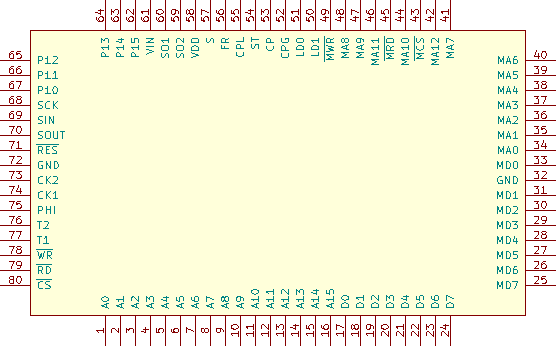
\includegraphics{DMG-CPU-pinout}
  \caption{DMG/SGB CPU (Sharp QFP080-P-1420)}
\end{figure}

\begin{figure}[H]
  \centering
  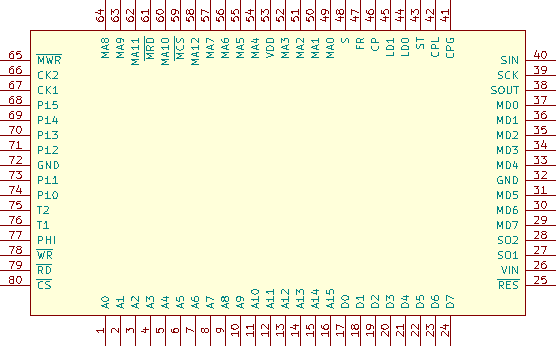
\includegraphics{MGB-CPU-pinout}
  \caption{MGB/SGB2 CPU (Sharp QFP080-P-1420)}
\end{figure}

\section{Cartridge chips}

\begin{figure}[H]
  \centering
  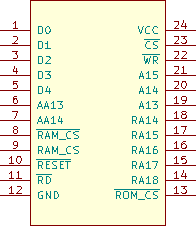
\includegraphics{MBC1-pinout}
  \caption{MBC1 (Sharp SOP24-P-450) \cite{tauwasser_mbc1}}
\end{figure}

\begin{figure}[H]
  \centering
  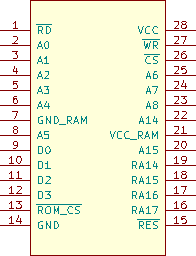
\includegraphics{MBC2-pinout}
  \caption{MBC2 (Sharp SOP28-P-450) \cite{tauwasser_mbc2}}
\end{figure}

\begin{figure}[H]
  \centering
  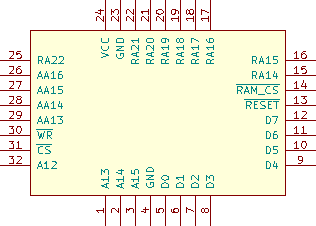
\includegraphics{MBC5-pinout}
  \caption{MBC5 (Sharp QFP32-P-0707)}
\end{figure}

\end{document}

\end{appendices}

\bibliography{gbctr}

\end{document}
